\documentclass[../main.tex]{subfiles}
\externaldocument{introduction}
\graphicspath{{\subfix{../images/}}}

\begin{document}

\subsection{Overview}

The overview of the proposed solution is depicted in 
\cref{fig:solution-overview}. 
The hardware components consist of an \anafi drone,
a Raspberry Pi with an external battery, and a Wi-Fi
dongle. The built-in camera of the drone is used to
take pictures of the targets and the Wi-Fi dongle
is used to communicate with the command and control
system, which sends high-level commands whenever the
connection is present. An object detection model trained
using RoboFlow detects and identifies the targets in the
pictures. In addition, a \gls{drl} agent is trained 
in a cyber-physical simulator called Sphinx to
visit virtual targets having the same mobility pattern as the
real ones.
This trained model is loaded into the Raspberry Pi that acts
as an onboard computer to the \anafi drone and instructs
it where to move to cover the targets in a minimum amount
of time.

The following subsections will
explain in more detail why this solution is chosen
and what the integral components are.

\begin{figure}[tbp]
	\centering
	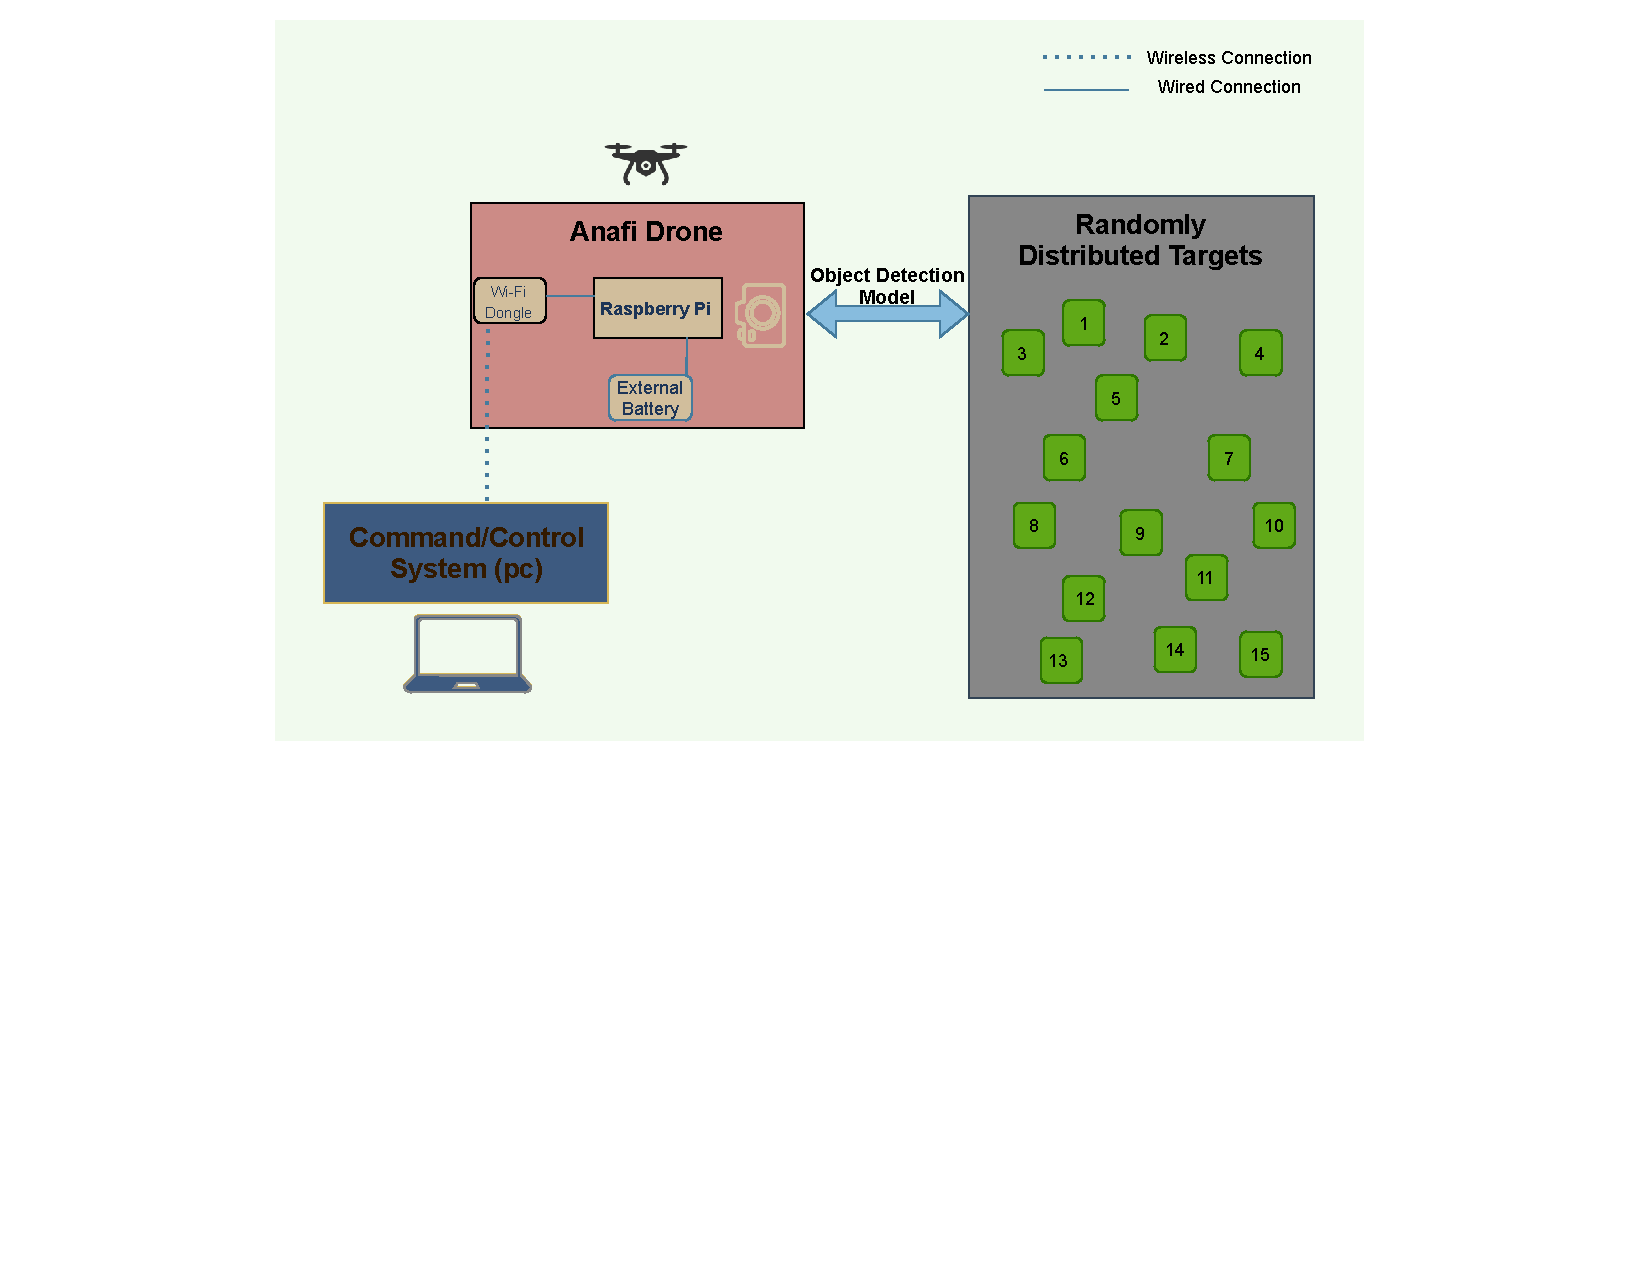
\includegraphics[width=0.9\textwidth]{solution-diagram}
	\caption{A general overview of the solution.}
	\label{fig:solution-overview}
\end{figure}

\subsection{High level architecture}

\Cref{fig:arch-fig} shows a high-level architecture 
of the complete working system, in which a group 
of connected adapters and devices are combined into 
a single functional system. 
The architecture is composed of three sections namely
interfacing, controlling, and targets. 
The interfacing section contains the drone that 
will handle the onboard computer, its power source, 
and the connection adapters. 
In the controlling part, a personal computer 
will be responsible for contacting the onboard computer 
to adjust settings, execute scripts, and get 
live updates and results. 
Finally, there are multiple moving targets 
in the target section. For example, 
\gls{rc} cars are controlled manually and move in 
a specific mobility pattern with varying directions 
and destinations. 
In the next section, hardware and software components 
will be presented in a more detailed manner.

\begin{figure}[h]
    \centering
    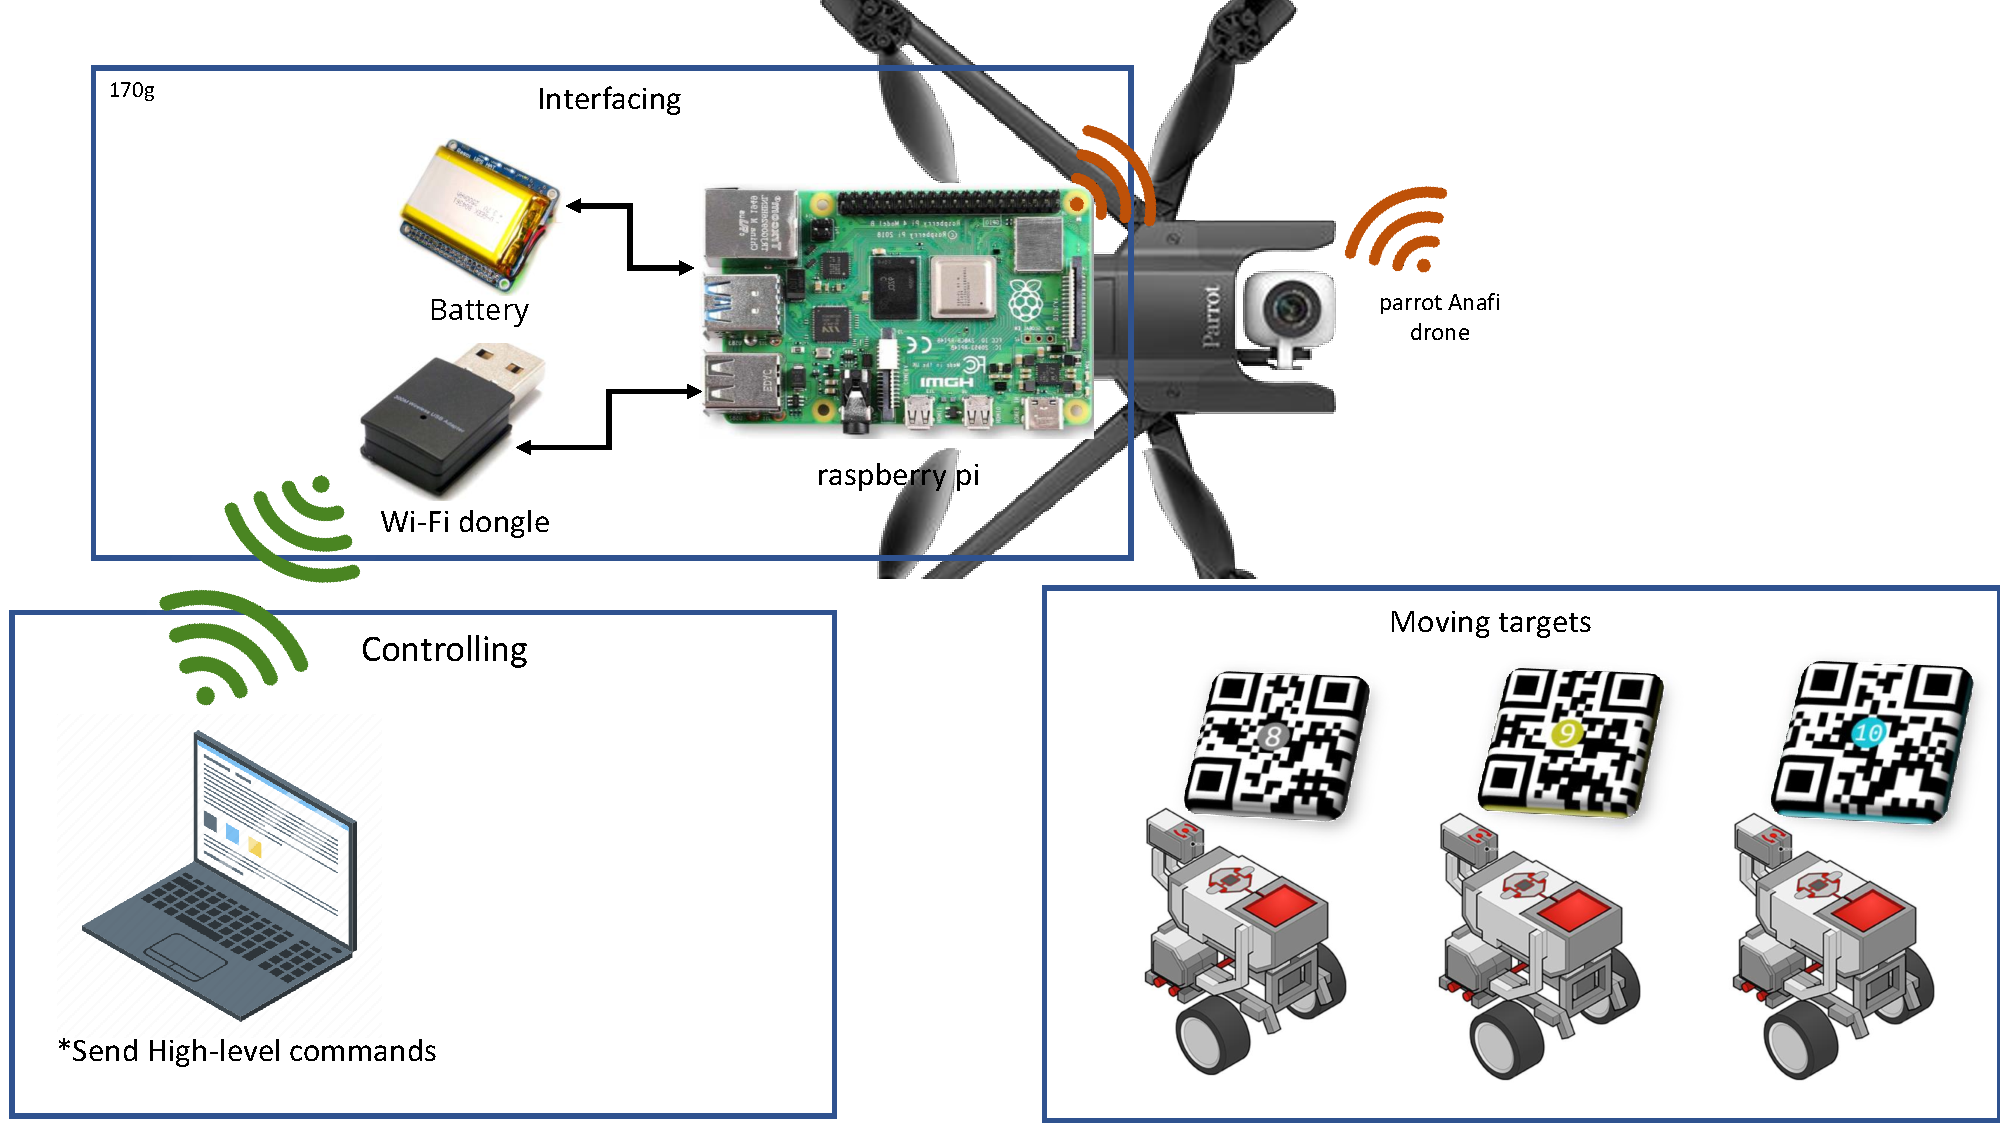
\includegraphics[width=0.9\textwidth]{high-level-arch.pdf}
    \caption{The high-level architecture of the overall system.}
    \label{fig:arch-fig}
\end{figure}

\subsection{Hardware/software used}

\subsubsection{Software}

There are three primary categories of software 
depending on the usage: simulation, training, 
and application, and they are listed in \cref{tab:software-used}. The first part will focus on 
simulating the environment, testing the models, 
and flight control. Before discussing the software 
to be used, we have selected Ubuntu 18.04 (Bionic Beaver) 
as an operating system for several reasons. 
One key reason is that in addition to
still being supported, it is compatible with the 
Parrot's Olympe and Sphinx programs, which are only 
supported on limited distributions and operating systems.
Another reason is that it is a lite \textsc{os} 
and can be installed on the onboard computer that 
will be attached to the drone. For the simulation part, 
using Sphinx and Gazebo software is very helpful
to visualize the environment, control the drone, 
and apply the \gls{drl} model. 

\begin{table}[p]
    \centering
    \caption{Software used in the project.}
    \label{tab:software-used}  
    \begin{tabular}{ p{3cm} p{3cm} p{6cm} }
        \toprule
        \textit{Software} 
            & \textit{Logo} 
                & \textit{Justification} \\ 

        \midrule

        Parrot Olympe  
            & 
            \raisebox{-0.7\height}
            {
\includegraphics[width=2.7cm]
            {parrot.png}}
                & A controller for the Parrot \anafi 
                drone. It makes controlling 
                the drone possible 
                using a Python script \\
                \addlinespace

        Parrot Sphinx  
            & 
            \raisebox{-0.7\height}
            {
\includegraphics[width=2.7cm]
            {parrot.png}}
                & A simulator for the Parrot \anafi drone.
                It loads the Parrot's drone firmware 
                in the simulation environment.
                It is largely based on Gazebo. \\
                \addlinespace

        Jupyter Notebook  
            & 
            \raisebox{-0.9\height}
            {
\includegraphics[width=2.5cm]{jupyter.png}}
                & A web application for writing, testing 
                and sharing of code. It is free 
                and does not require internet access like 
                the Google Colab. It is used heavily 
                in this project to experiment with new 
                ideas in the Sphinx simulation. \\ 
                \addlinespace

        Zbar
            & 
            \raisebox{-0.9\height}
            {
\includegraphics[width=1.8cm]{zbar.png}}
                & A software suite capable of reading widely-used
                symbologies including QR code. Its Python binding
                Pyzbar is used as a library in this project to
                detect the QR codes of the targets. \\ 
                \addlinespace
		Python Flask
		& 
		\raisebox{-0.9\height}
		{
\includegraphics[width=2.8cm]{flask-logo}}
		& A backend framework written in python, 
		it does not require any libraries or tools 
		which qualifies it as a microframework. 
		%It has a built-in web server, but it is not suitable
		%for production, so it is best used with a 
		%\textsc{wsgi} \textsc{http} server. 
		\\ 
				\addlinespace
		Gunicorn
		& 
		\raisebox{-0.9\height}
		{
\includegraphics[width=2.8cm]{gunicorn-logo}}
		& A Python Web Server Gateway Interface \textsc{http} server.
		It is very commonly used for web app deployment as it implements 
		\textsc{pep} 3333 Python \textsc{wsgi} interface.
		
				\\ 
				\addlinespace				
		Nginx
		& 
		\raisebox{-0.9\height}
		{
\includegraphics[width=2.8cm]{nginx-logo}}
		& A web server that can be utilized in many different ways. Mainly, a 
		reverse proxy, mail proxy, \textsc{http} cache, and a load balancer. 
		It is very wildly used as it has outperformed Apache due to its 
		scalability and lightweight.
		\\ 
		\addlinespace
		
        \bottomrule
    \end{tabular}
\end{table}

Sphinx is a simulation 
tool built on top of Gazebo 
to run the Parrot's drone firmware on 
personal computers, which comes with helpful 
features for simulation such as visualizing flight 
data at runtime, running the \gls{uav} remotely, 
and executing scripts with the command line. 
Gazebo is a robot \textsc{gui} simulation 
which simulates the visual and physical surrounding 
of drones and custom 3D objects. 
\Cref{fig:gazebo} shows how the Sphinx 
program looks like. 

\begin{figure}[tbp]
    \centering
    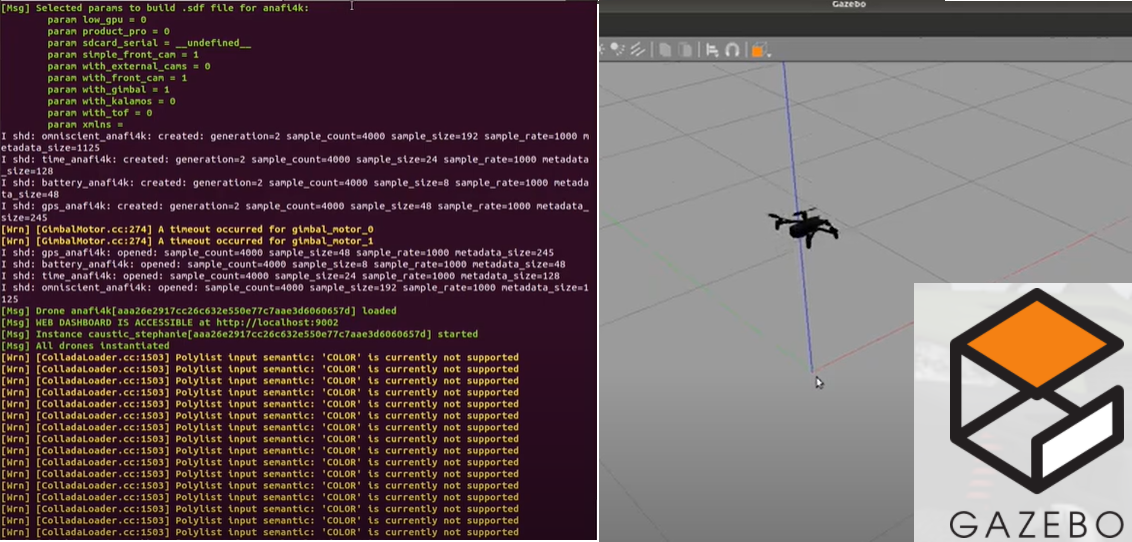
\includegraphics[width=0.9\textwidth]{gazebo.png}
    \caption{The Sphinx program that runs on top of Gazebo.}
    \label{fig:gazebo}
\end{figure}

For the object detection model, the Pyzbar library was used to detect
the QR codes of the targets.
It has an accuracy of up to 90\% in good conditions but can be as
low as 30\% when the QR code is damaged due to an error in photo
capturing and processing~\cite{dynamsoft}.

For the application software, Parrot Olympe 
was used to send commands to the physical as well as 
the simulated drone and control the flight trip and 
how the drone moves. Parrot Olympe uses Python 
controller programming interface for Parrot drones 
which makes controlling simple and easy using a 
Python script. Moreover, Olympe allows us to read
sensor data, such as the \gls{gps} fixes and camera feed, 
from the \anafi
drone. This will make it possible to build a user interface
on the control and command station to monitor 
the progress of the drone
when it is autonomously executing the task visitation
mission.



\subsubsection{Hardware}

The main core of the hardware part is the drone, 
which will be the Parrot \anafi.
\Cref{tab:hardware-used} lists the hardware components
used in this project and their justifications. This quad-copter
drone is powerful because it combines many technologies 
and sensors in a small foldable size. It also it has 4K HDR Camera supported 
with 180 degree gimbal. 
There are seven sensors in total inside the drone which are shown in 
\cref{tab:sensors-table} 


\begin{table}[H]
	\centering
	\caption{Processor and sensors inside the drone}
	\label{tab:sensors-table}  
	\begin{tabular}{ p{4cm} p{8cm} }
		\toprule
		\textit{Part Name} 
		& \textit{used for}  \\ 
		
		\midrule
		Ambarella H22 
		processor
		& powerful Quad-core ARM® Cortex™ - capable of dealing with sensors and video I/O , 
		image processing , video encoding , interfacing \\ 
		3-axis gyroscope
		& measure the orientation and angular velocity  \\ 
		3-axis accelerometer
		& measure the acceleration in 3 dimensions  \\ 
		magnetometer 
		& measure the Earth's magnetic field to know the orientation and the heading   \\ 
				barometer 
		& measure atmospheric pressure change to control flight height   \\ 
				GPS 
		& determine the location of the drone and navigation  \\ 
				Ultrasonar 
		&  height measurement for small height less than 5 meters  \\ 
				Vertical camera 
		&  measuring horizontal speed and height using optical flow \\ 
        \bottomrule
    \end{tabular}
\end{table}   

The second important device is the Raspberry Pi 4 model B. It 
acts as an onboard computer and is used in this project
mainly to facilitate the low-level control of the drone
by sending frequent control commands to the drone
in a certain direction or stay hovering.
The choice of action is determined by the \gls{drl}
model that will be installed in it.
Hence, the tasks of the Raspberry Pi are: 

\begin{enumerate}
	\item connecting to the drone's access point 
	using a Wi-Fi interface,
	\item controlling the drone 
	by executing Olympe to send low-level control signals 
	and to receive sensory data,
	\item applying the \gls{drl} model supported by 
	the command and control system,
	\item receiving high-level commands and sending video 
	frames to the command-control system from the drone camera.
\end{enumerate}
 
The Parrot \anafi drone is connected 
to the Raspberry Pi, which is the onboard computer,
using both devices' internal 
\SI{2.4}{\giga\hertz}
Wi-Fi interfaces. 
Firstly, we add the \anafi drone's access point 
to the saved devices list in the Raspberry Pi.
Once the Raspberry Pi boots up, it automatically keeps 
searching for the access point and connects 
to it once it is available.

For the connection between the command and control system 
and the Raspberry Pi, 
the Raspberry Pi will use a 
\SI[per-mode=symbol,per-symbol=p]{300}{MBps} 
Wi-Fi adapter dongle connected to 
its \textsc{usb} port. 
This will allow it to create an access point to which 
the command and control device will connect and by which 
the Raspberry Pi can be controlled. This control of the 
onboard computer is done through the graphical user interface,
which is simply a web-based application 
that will allow the user to send the
control commands and receive the video frames. 


Regarding the power source for the Raspberry Pi, 
we considered taking power directly from the 
drone's battery, but after some research, we found 
that the \anafi drone's  
socket is somehow different in the type and the power output. It is also challenging 
because the drone battery is susceptible to shutting down 
immediately if the voltage reaches less than 3.0 Volt. 
Therefore, we did not want to take the risk so we used a 
lithium battery with a power board called 
\textsc{upsp}ack Standard Power Supply attached to 
the main Raspberry Pi board. It includes a 
\SI{4000}{\milli\ampere\hour}
lithium battery, which provides enough power 
and long-lasting time for our application.
\Cref{tab:hardware-used} lists the hardware components
used in this project and their justifications. 

Finally, in \Cref{fig:3d-design} we have designed a 3D printed case that 
will hold all the components above the drone in 
a stylish and professional way. We have considered two 
points in the design. The first one is the weight and the minimal
complexity, as we have a limited payload that the drone 
can lift and a narrow space that can fit above the drone.
The second point is that the Raspberry Pi usually 
becomes hot due to processing and usage, so we need 
a design that will help the airflow go through and keep 
the ventilation process, and this is why we have 
the holes in the case design.   

\begin{figure}[h]
	\centering
	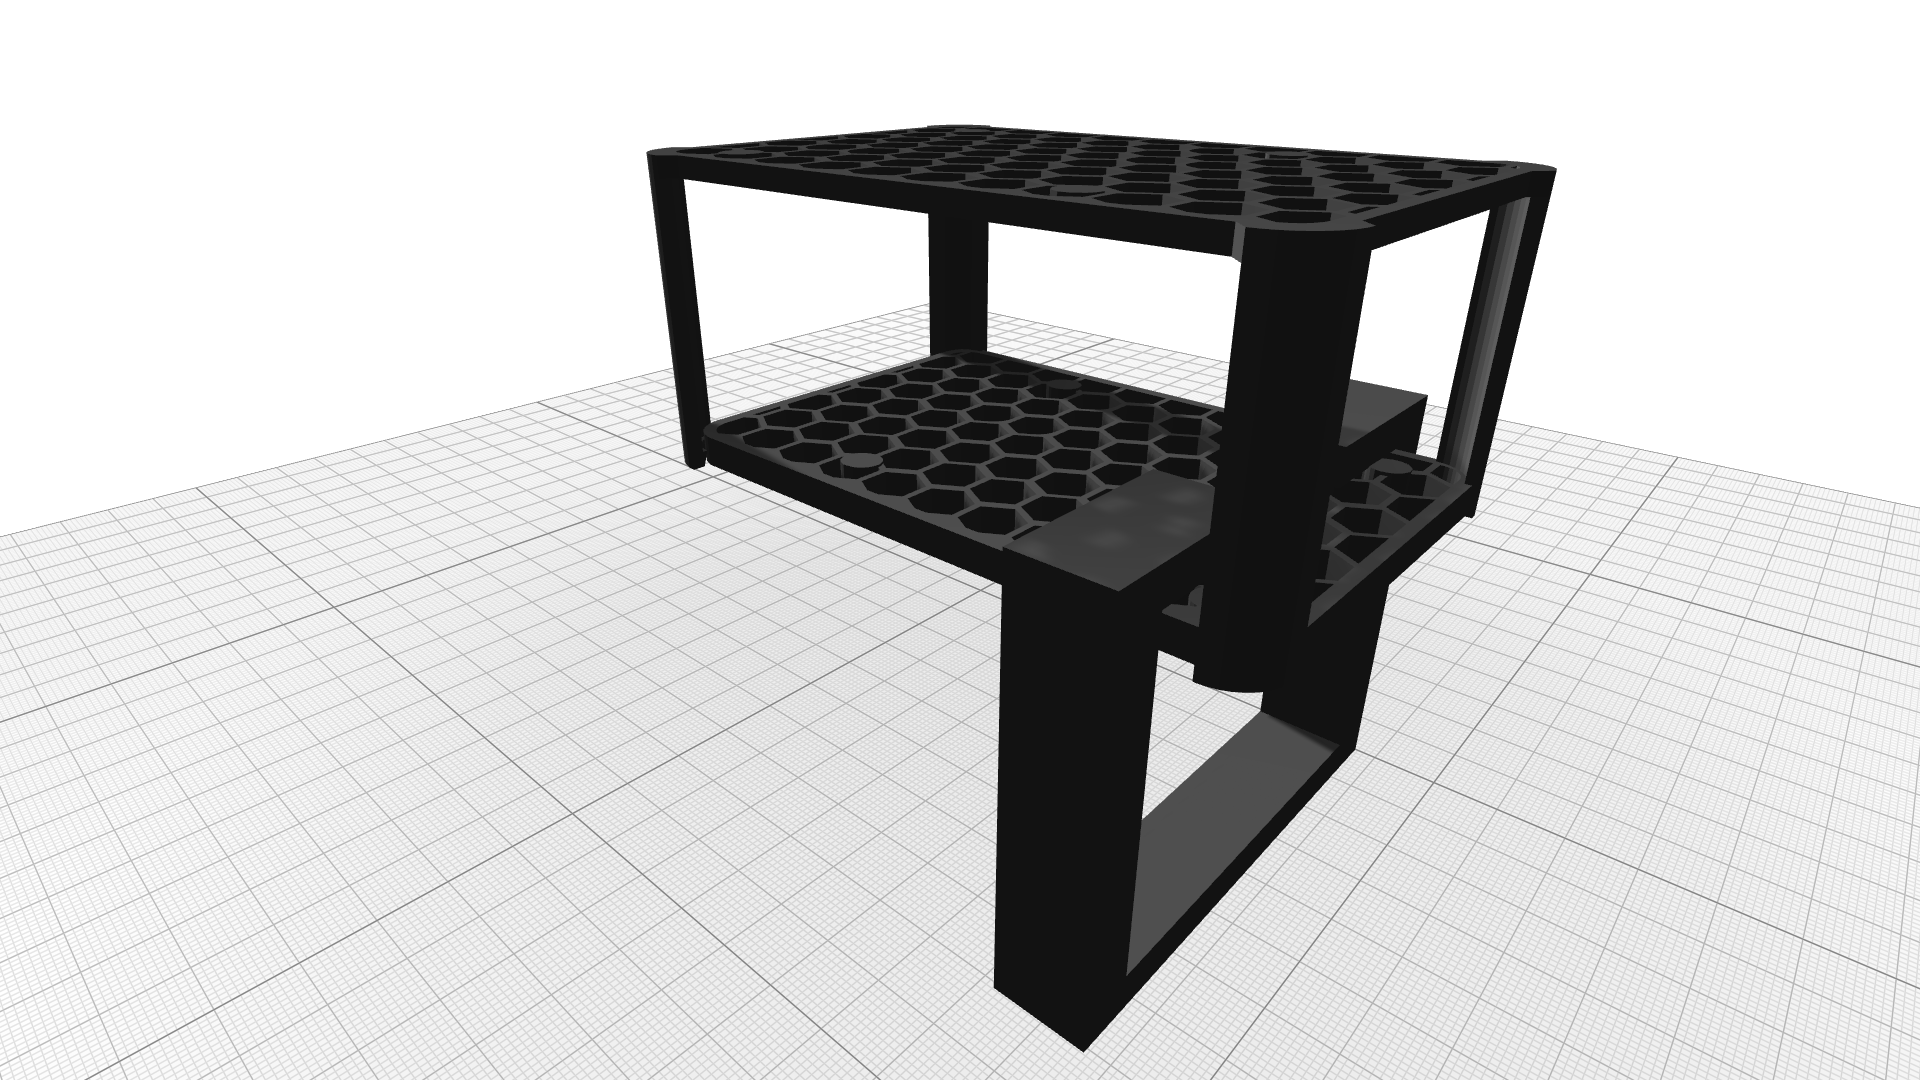
\includegraphics[width=0.9\textwidth]{3d-model-design.png}
	\caption{3D design of the onboard computer case.}
	\label{fig:3d-design}
\end{figure}


\begin{table}[p]
	\centering
	\caption{Hardware used in the project.}
	\label{tab:hardware-used}  
	\begin{tabular}{ p{4cm} p{3cm} p{6cm} }
		\toprule
		\textit{Hardware} 
		& \textit{Picture} 
		& \textit{Justification} \\ 
		
		\midrule
		
		Parrot \anafi Drone  
		& \begin{minipage}{.1\textwidth}
			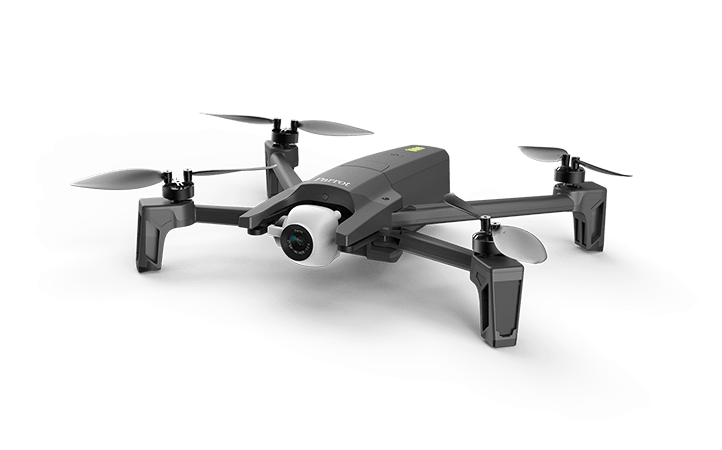
\includegraphics[width=30mm, height=20mm]{anafi.png}
		\end{minipage} 
		& Available in the university, can be 
		controlled easily 
		with simple Python script, 
		4K-high resolution camera.  \\ 
		\addlinespace
		
		Raspberry Pi 4  
		& \begin{minipage}{.0\textwidth}
			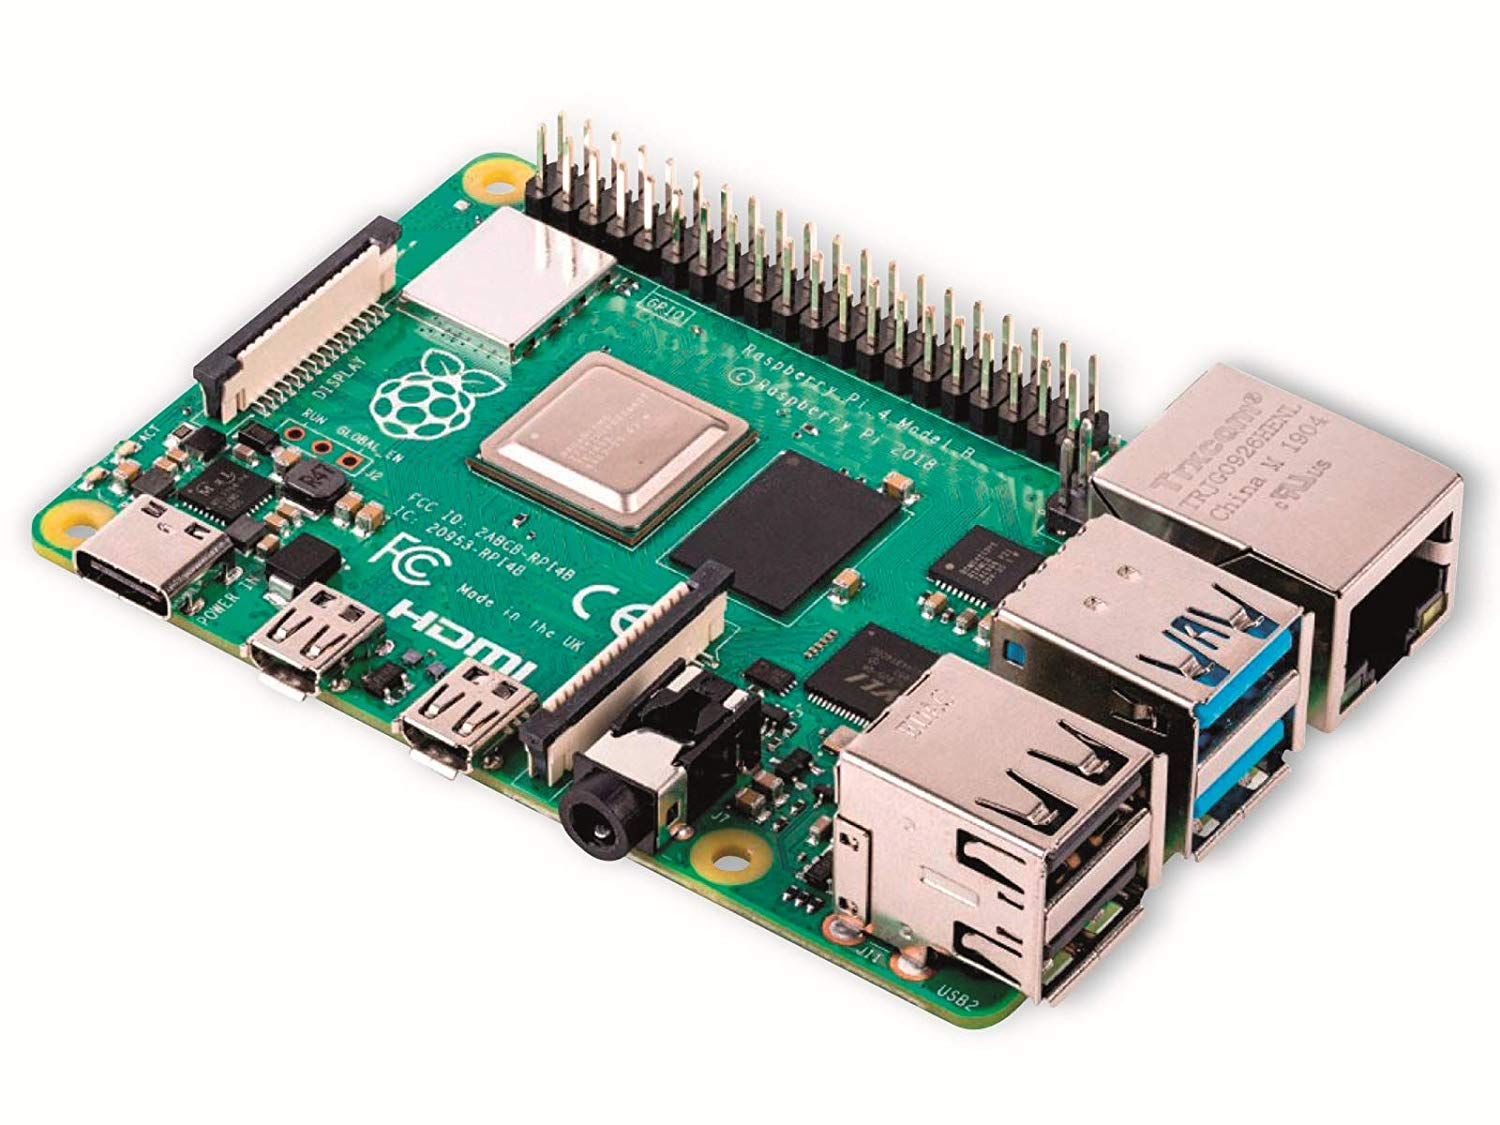
\includegraphics[width=30mm, height=20mm]{raspberry.jpg}
		\end{minipage} 
		& Specifications are enough for our 
		application, support Wi-Fi and its 
		small size and weight is an advantage.\\ 
		\addlinespace
		
		\textsc{rpi} \textsc{upsp}ack \textsc{v}3 with 
		\SI{4000}{\milli\ampere\hour} 
		lithium Battery  
		& \begin{minipage}{.1\textwidth}
			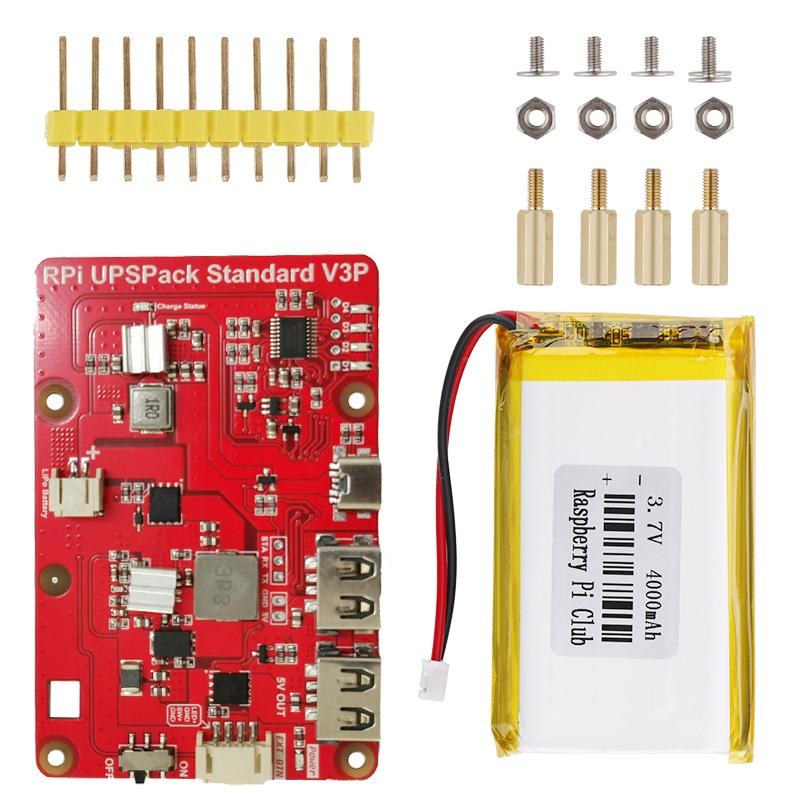
\includegraphics[width=30mm, height=35mm]{RPI.jpg}
		\end{minipage}  
		& Support up to 4 hours which is more 
		than enough , the board got an \textsc{led} 
		indicator for charging level also the 
		weight and shape is an advantage.  \\ 
		\addlinespace
		
		Wireless N Nano \textsc{usb} Adapter  
		& \begin{minipage}{.1\textwidth}
			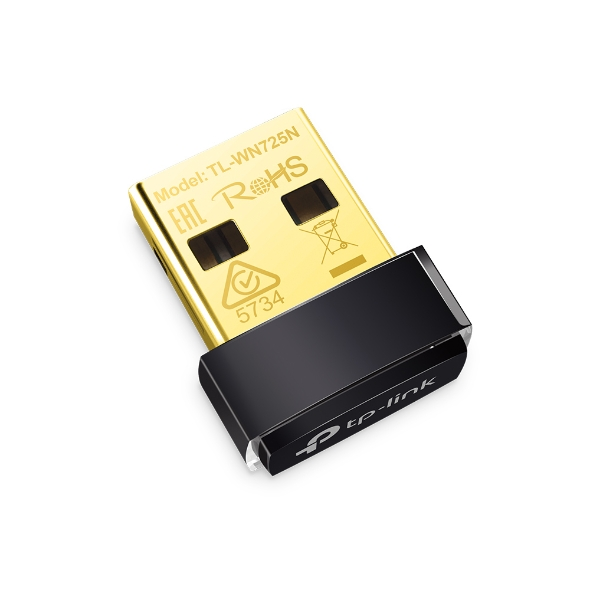
\includegraphics[width=28mm, height=28mm]{dongle.jpg}
		\end{minipage} 
		& Cheap and do its job, good coverage 
		range.  \\ 
		\addlinespace
		
		Laptop 
		& \begin{minipage}{.1\textwidth}
			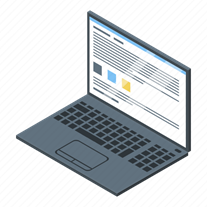
\includegraphics[width=30mm, height=30mm]{laptop.png}
		\end{minipage} 
		& Any laptop with good WiFi interface 
		card will be enough for our case. \\ 
		\addlinespace
		
		\bottomrule
	\end{tabular}
\end{table}


\subsection{Hardware design}

\subsubsection{UAV options}
\begin{table}[H]
	\centering
	\caption{A comparison of the \gls{uav} options.}
	\label{tab:alt-solutions}
	\begin{tabularx}{\textwidth}{ p{4cm} X X }
		\toprule
		\textit{} & \textit{Option A} & \textit{Option B}\\ \midrule
		Type  & Custom made drone with onboard computer & 
		Commercial drone with high performance and many features    \\
		Flexibility & Very flexible and customization is easy & 
		Hard to customize or modify it since it flies under 
		limited protocols and standards. \\
		
		Price and Availability & Cheaper but the shipping and 
		building processes must be considered & Expensive but 
		in our case its available in our hands and ready to fly.   \\
		
		Onboard computer & Must have & Must have \\
		\bottomrule
	\end{tabularx}
\end{table} 

In \cref{tab:alt-solutions}, 
we can see some trade-offs 
between option A and option B. However, in both designs, 
an onboard microcomputer must be present for 
flying control and the for the support of autopilot feature as well as for 
transmitting the video frames. 


Firstly, developing a custom drone will consume a lot of time and effort, 
which is different from our design project idea.
Hence, we have chosen the commercial drone option especially 
the Parrot \anafi for several reasons.
The fact that it is supported by a continuously updated 
\textsc{sdk} and can be controlled easily 
with a simple Python script makes 
\gls{drl} development much easier and more stable among common reasons.

Secondly, it has a good flight time 
as the \anafi drone has a 2700 mAh battery. 
It can fly up to 25 minutes, which is good enough 
for our application.
Finally, its support of Wi-Fi 802.11 and \gls{gps} 
features is essential in our project for 
executing scripts and navigation.

\subsubsection{Onboard-computers options}
There are three options for onboard microcomputers, 
which are shown in the following 
\cref{tab:onboard-computers}. Raspberry Pi 4 seems 
to be the best option since it has advantages 
in specifications, connection interfaces, 
and availability.

\begin{table}[H]
	\centering
	\caption{A comparison of the onboard computers.}
	\label{tab:onboard-computers}  
	\begin{tabular}{ p{3cm} p{4cm} p{4cm} p{4cm} }
		\toprule
		\textit{} & \textit{Raspberry Pi 4} & \textit{\textsc{nvidia} Jetson Nano} & 
		\textit{\textsc{dji} Manifold}\\ \midrule
		Specifications  & \textsc{cpu}: Cortex-A72 (\textsc{arm} v8) 64-bit@ 1.5GHz | Ram: 4GB or 8GB \textsc{lpddr4}-3200 \textsc{sdram} | \textsc{gpu}: Broadcom VideoCore VI & 
		\textsc{cpu}: Quad-core \textsc{arm} A57 @ 1.43 GHz | Ram: 4 GB 64-bit 
		\textsc{lpddr4}   | \textsc{gpu}: 128-core Maxwell & \textsc{cpu}: Quad-core, 
		\textsc{arm} | Ram: 2 GB \textsc{ddr3l} | \textsc{gpu}: Low-power GeForce
		 graphics processor \\ \addlinespace
		Connection interfaces & 2.4 GHz and 5.0 GHz \gls{ieee} 802.11ac wireless,
		 Bluetooth 5.0 & Gigabit Ethernet \& M.2 Key E (for WiFi support). &10/100/1000 
		 \textsc{base-t} Ethernet \\ \addlinespace
		
		Price \& Availability & \qar{300}. Available and can be used on any drone & 
		\qar{400}. Available but needs to be ordered and shipped & Very expensive 
		and restricted to \textsc{dji} drones and \textsc{dji} company stopped 
		selling it \\ \addlinespace
		Picture & \begin{minipage}{.2\textwidth}
			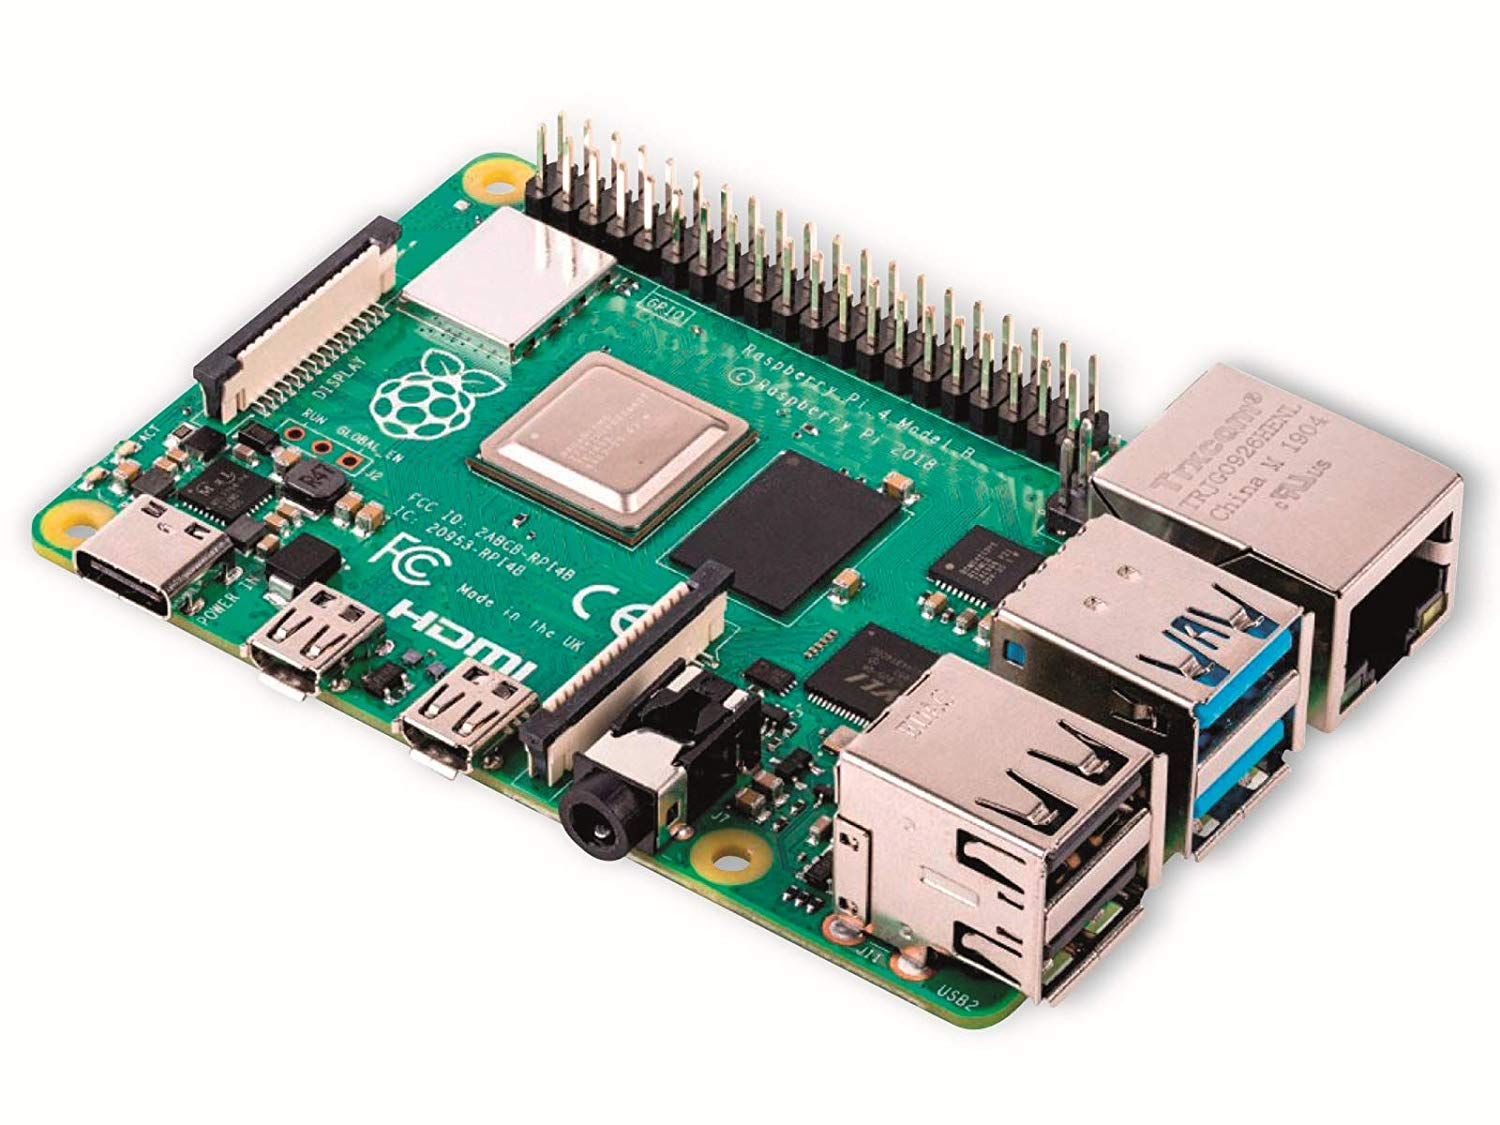
\includegraphics[width=40mm, height=30mm]{raspberry.jpg}
		\end{minipage}  & \begin{minipage}{.2\textwidth}
			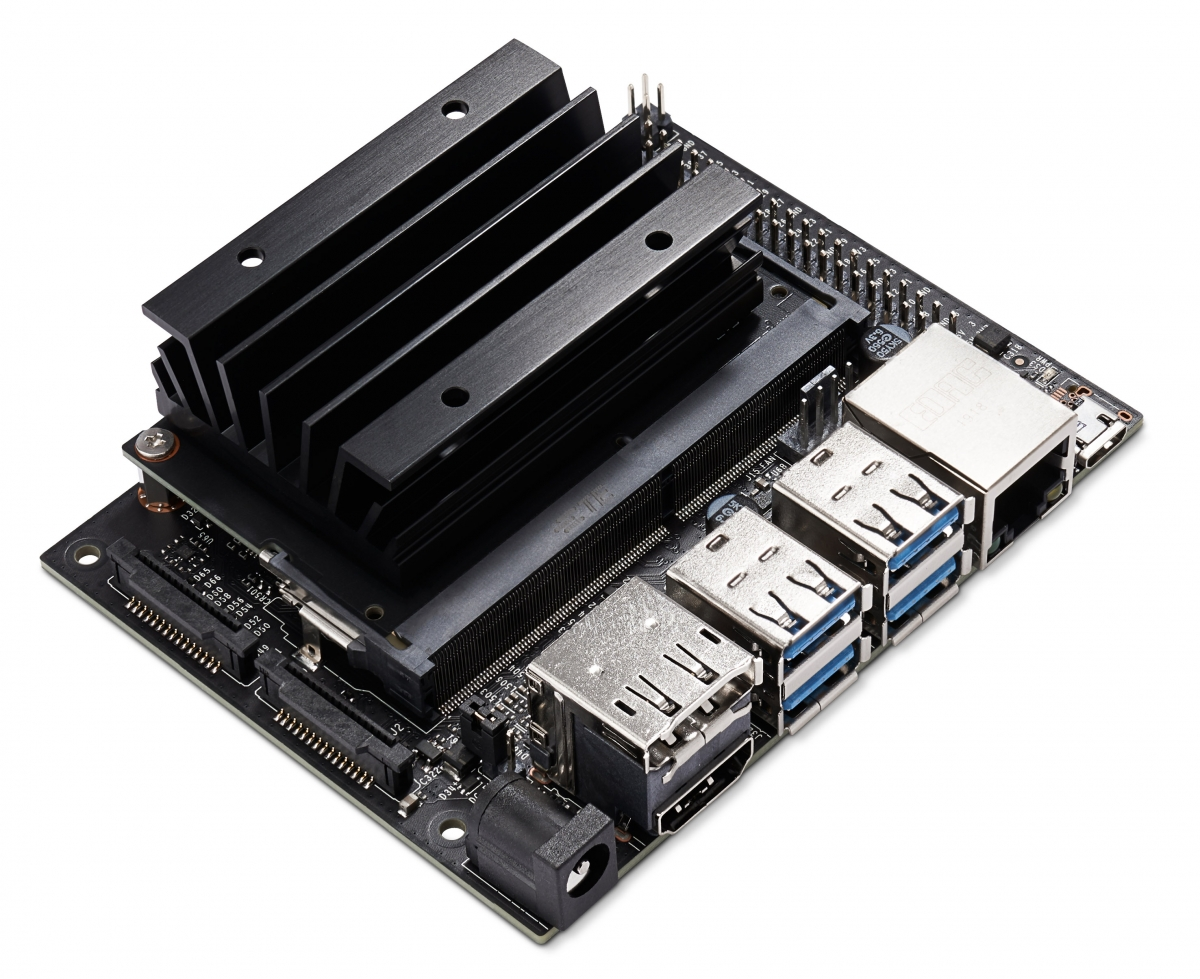
\includegraphics[width=40mm, height=30mm]{jetson.jpg}
		\end{minipage} & \begin{minipage}{.2\textwidth}
			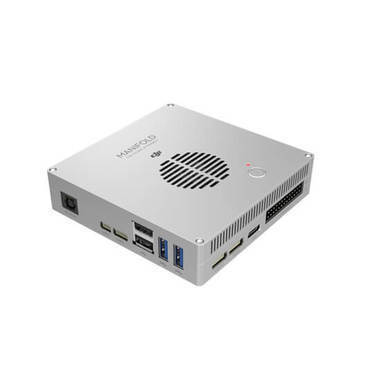
\includegraphics[width=40mm, height=30mm]{manifold.jpg}
		\end{minipage} \\
		\bottomrule
	\end{tabular}
\end{table}

\subsubsection{Power Supply options}
As shown in \cref{tab:power-sources}, there are different options for
the raspberry pi power sources, we have chosen the second option
RPI pack because it is a complete package and lightweight compared 
to other options; availability was also another primary concern. 
\begin{table}[H]
	\centering
	\caption{A comparison of the Power-supply sources for RPI4.}
	\label{tab:power-sources}  
	\begin{tabular}{ p{3cm} p{4cm} p{4cm} p{4cm} }
		\toprule
		\textit{} & \textit{UPS HAT Stable \& Lithium ion battery} & 
		\textit{RPI-ups-pack Lithium polymer battery} & \textit{Power bank}\\ \midrule
				Weight & 80g & 70g & 1.2kg \\ \addlinespace
				Voltage,current & 5V 3.5A  & 5V 3.5A &  5V 3.5A\\ \addlinespace
				
				Price \& Availability & \qar{100}.board available online without batteries & 
				\qar{80}. Available online with battery included & \qar{60}. available 
				locally\\ \addlinespace
				Charging duration  & longer & fast & longer \\ \addlinespace	
				Picture & \begin{minipage}{.2\textwidth}
					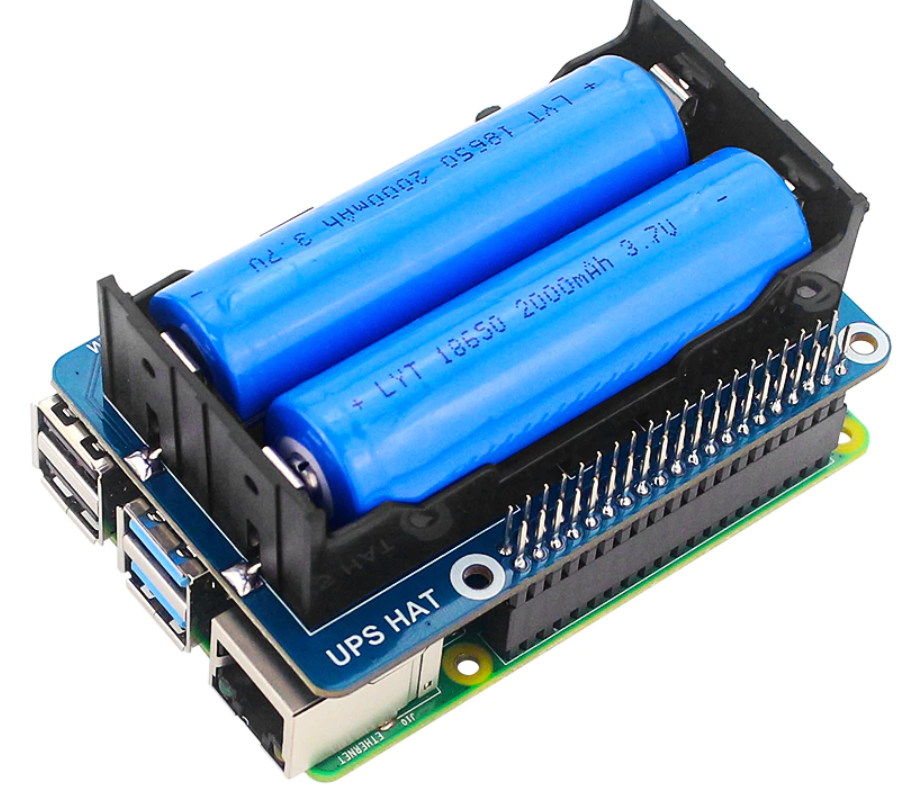
\includegraphics[width=40mm, height=30mm]{ion-battery-ups-haT.png}
				\end{minipage}  & \begin{minipage}{.2\textwidth}
					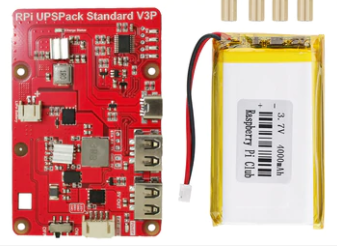
\includegraphics[width=40mm, height=30mm]{rpi-ups-pack.png}
				\end{minipage} & \begin{minipage}{.2\textwidth}
					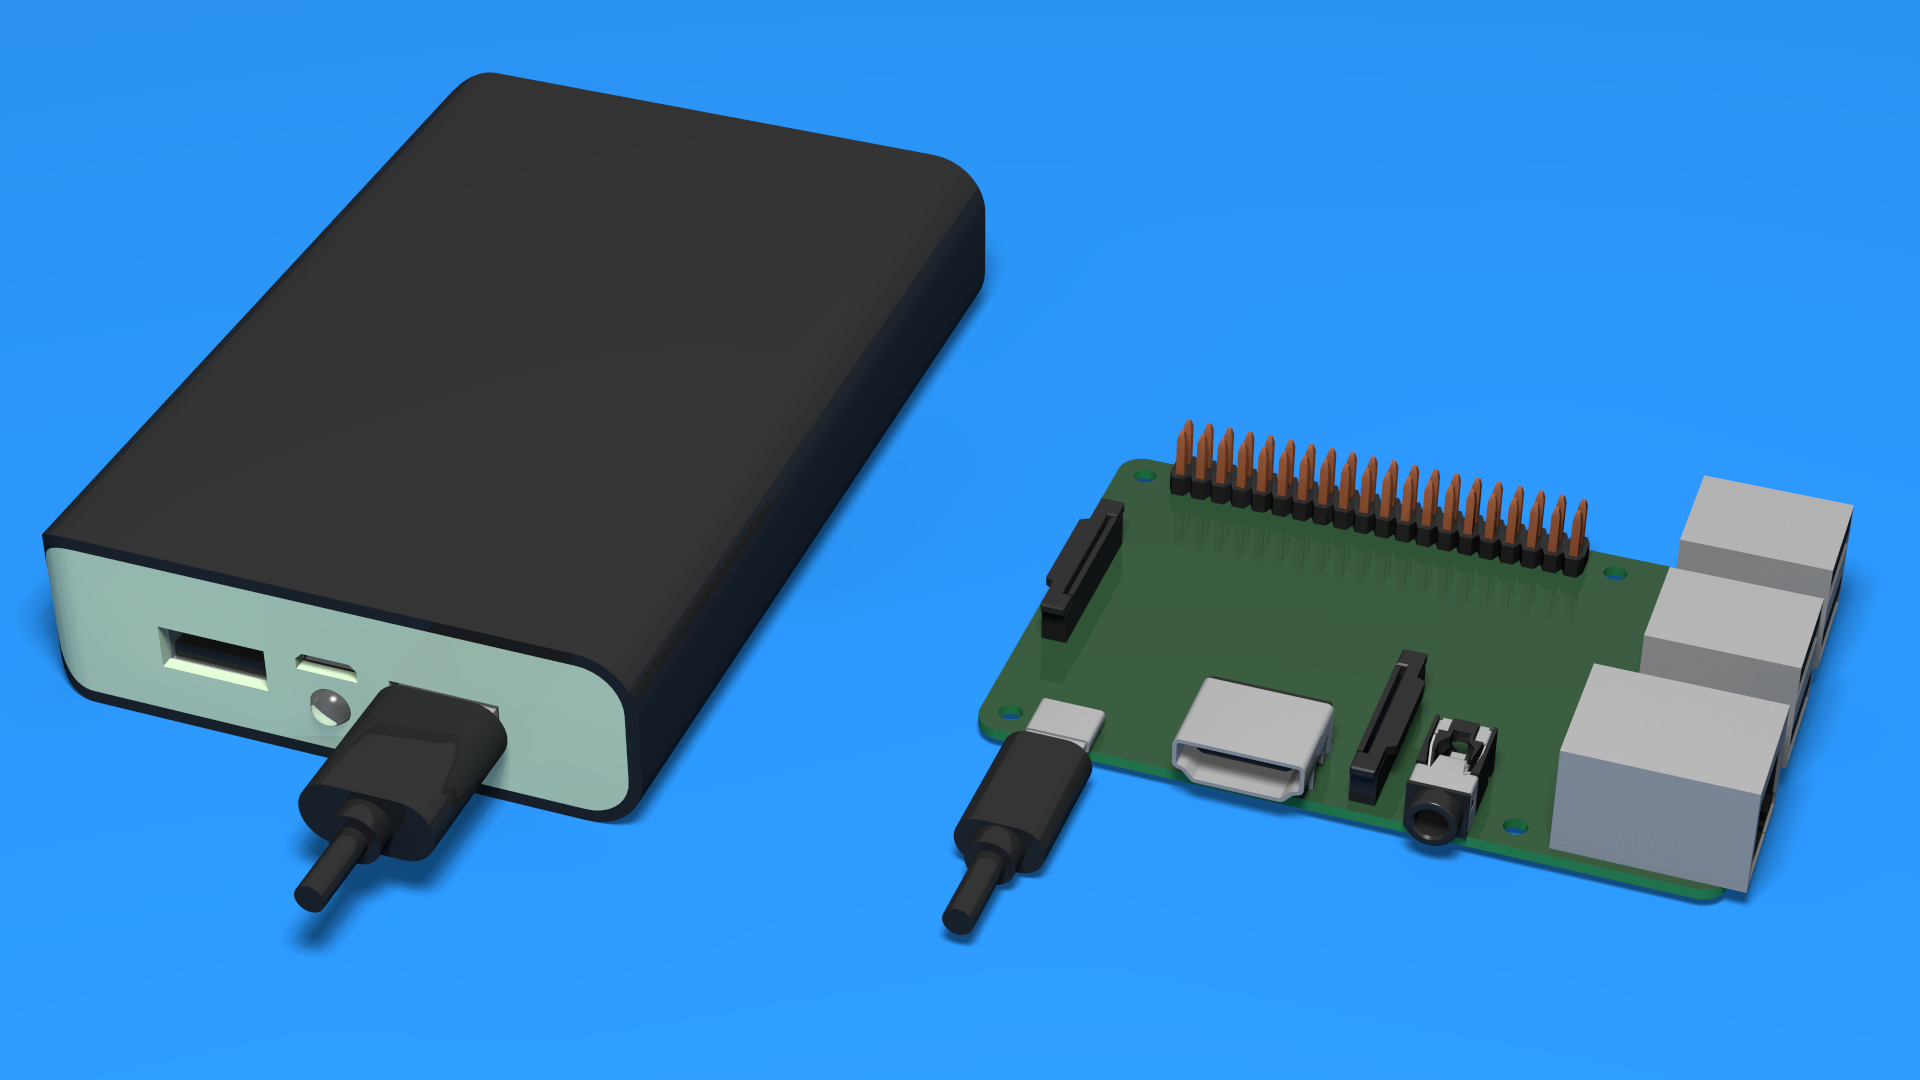
\includegraphics[width=40mm, height=30mm]{power-banks.png}
				\end{minipage} \\
				\bottomrule
			\end{tabular}
		\end{table}


	

\subsection{Software design}

\subsubsection{Simulation}
Based on the use case of this project, we first receive information
about the targets' count, distribution and mobility pattern and use
these pieces of
information to produce a file containing the weights for a \gls{drl}
model.
The simulation and \gls{rl} are critical
components to output this file thus achieving objective~\ref{obj:drl}.
The design for these components are shown in~\cref{fig:sim-flowchart}.

\begin{figure}[p]
    \centering
    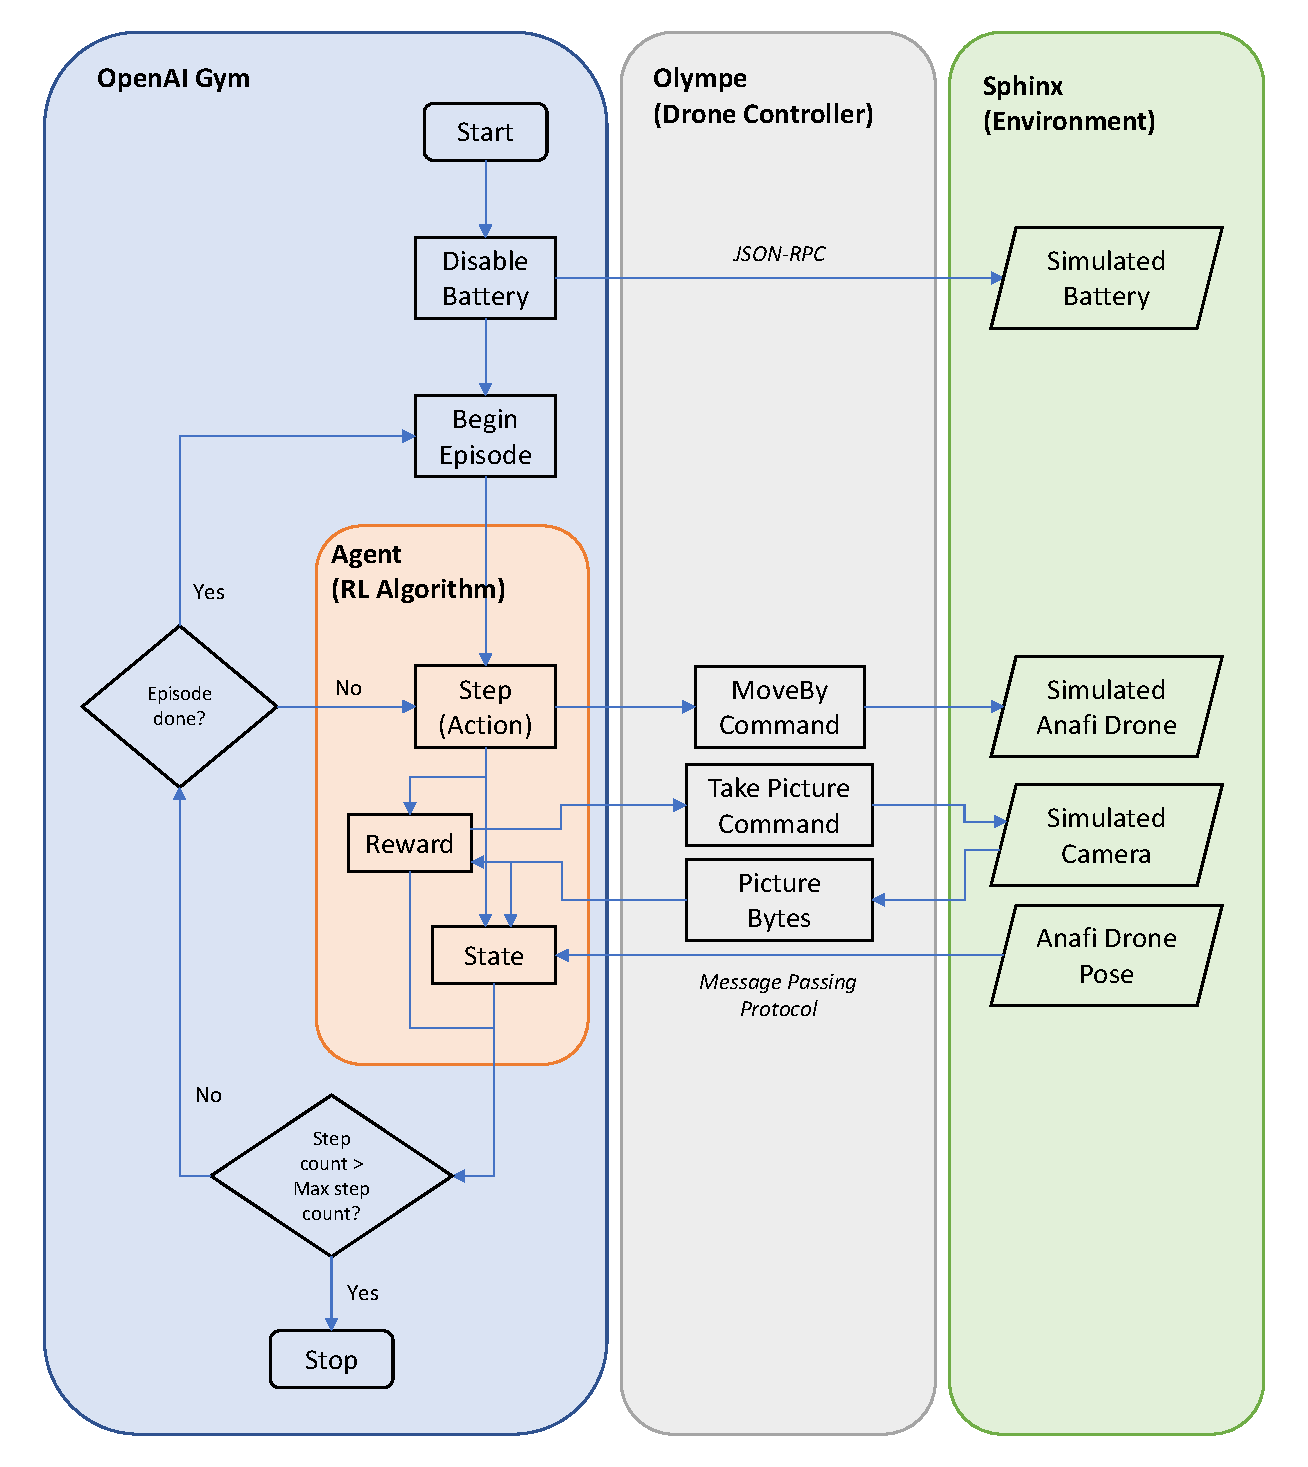
\includegraphics[width=1.0\textwidth]{sim-flowchart}
    \caption{A flowchart showing the training process
        of the \gls{rl} in the project
        and the interactions between the libraries
        and programs.}
    \label{fig:sim-flowchart}
\end{figure}

In our framework, we have used the Parrot Sphinx simulator
as the environment and a simulated Anafi drone as the agent.
The simulated drone extends the OpenAI Gym \texttt{Env} 
Python class
to inherit the methods every RL agent
needs to undergo to learn.
The exchange of state, reward and action between them 
occur through the Parrot Olympe controller as well as
through JSON-RPC and message passing protocols.
More detailed commands used and steps taken are laid out 
in~\cref{fig:sim-flowchart}.

The Parrot Olympe library was used for sending movement commands to
the drone.
It allowed us to connect
to the simulated drone by specifying the drone's
\textsc{ip}. Once the connection was established, 
we could send the Olympe control commands to the drone
to execute the visitation task. 
Which command to use
depends on the \gls{rl} model.

The \gls{rl} was aided 
by another library called \gym.
We used it to facilitate developing the
\gls{drl} algorithm we are implementing and to 
teach the drone how to achieve the 
target visitation mission.
Specifically, \gym provides an abstract class 
called \texttt{Env}
which we have inherited and overridden the 
required methods.
One of the methods is step() which is contained in
\cref{fig:sim-flowchart}.

To train a drone using RL requires the
design of the environment, the agent itself and
the interaction between them as shown in~\cref{fig:rl}. 
The agent, due to being in a certain state, chooses and 
performs an action on
the environment resulting in the environment 
rewarding the agent for taking the action in that state
and then replying to it with a next state.

\begin{figure}[!t]
	\centering
	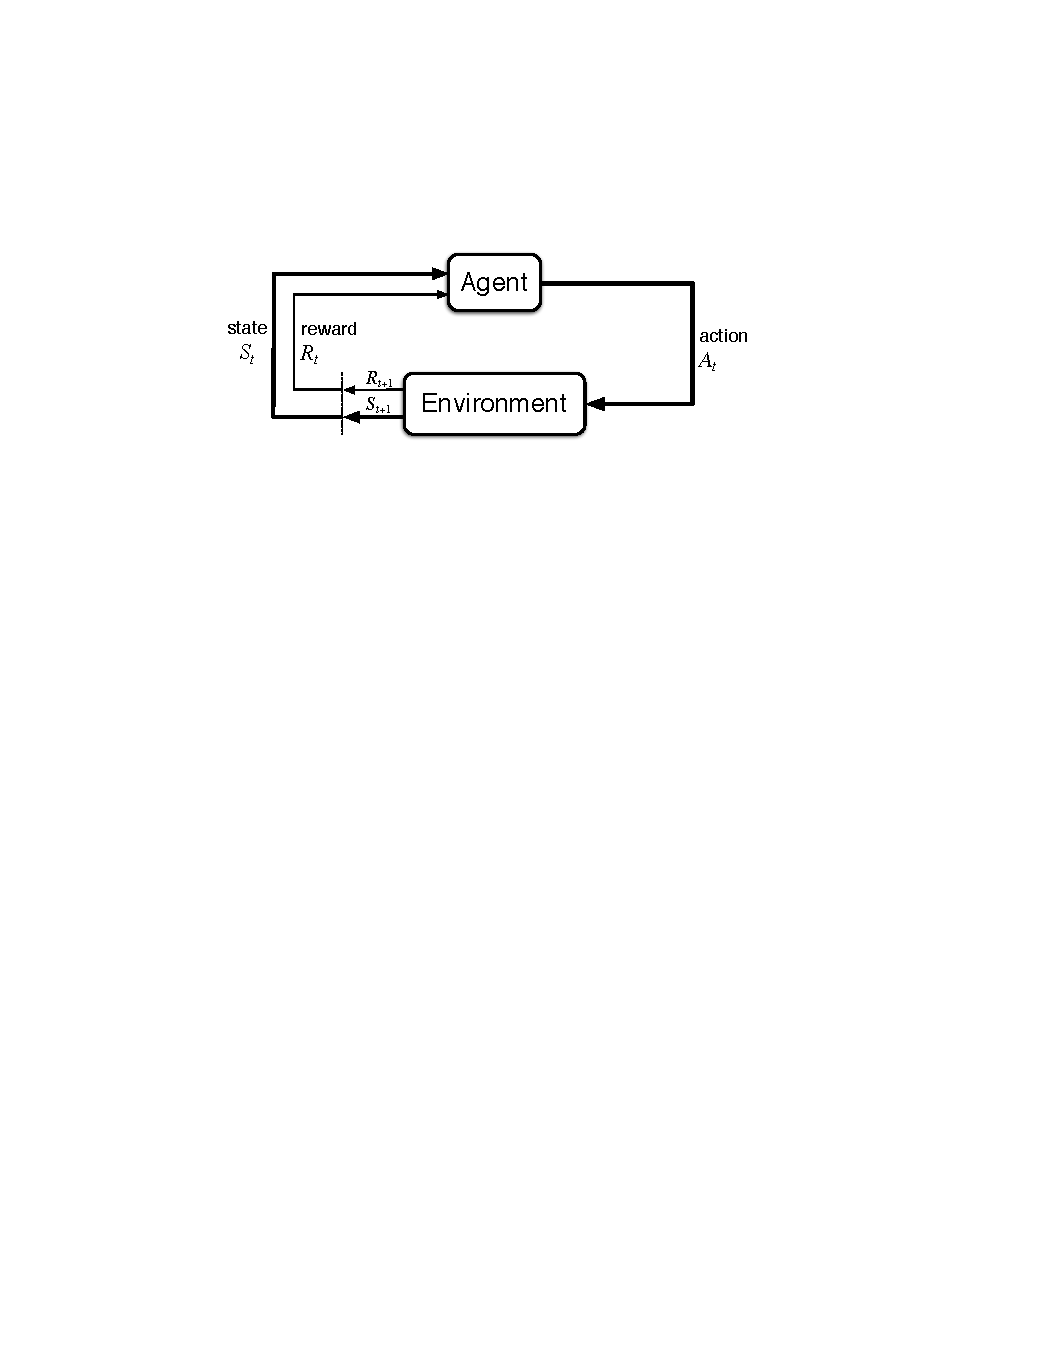
\includegraphics[width=0.8\textwidth]{rl-flowchart}
	\caption{The interaction between the agent and environment
        in \gls{rl} \cite{Sut20}.}
	\label{fig:rl}
\end{figure}

The action space of the agent is defined as a class, and its
elements call the necessary Olympe functions. 
The space consists of 9 movements: 
forward, backward, left,
right, forward-left, forward-right, backward-left,
backward-right and no-operation (hover).

We have set the reward to be equal to 1.5 multiplied by 
the number of new targets captured in the new state.
Each target is given a unique \textsc{id} which 
is embedded in the \textsc{qr} code that the targets are covered with
as shown in~\cref{fig:target}.
If there is no new target, the reward is -1. 
This ensures the drone learns to
minimise the time.
Since there are 10 targets, it follows that the maximum
return (sum of rewards in an episode) that the agent can gain  
in an episode is 
\begin{align}
        1.5 \times 10 = 15
\end{align}
To obtain the number of new targets, the drone's simulated camera is
used to take a photo of the cell
underneath, which is then processed by a \textsc{qr} code detection 
model, Pyzbar. 
The outputs of the processing are the \textsc{id}s of 
the detected targets, 
of which only the previously not encountered ones during 
the episode are counted towards the reward.

\begin{figure}[!t]
	\centering
	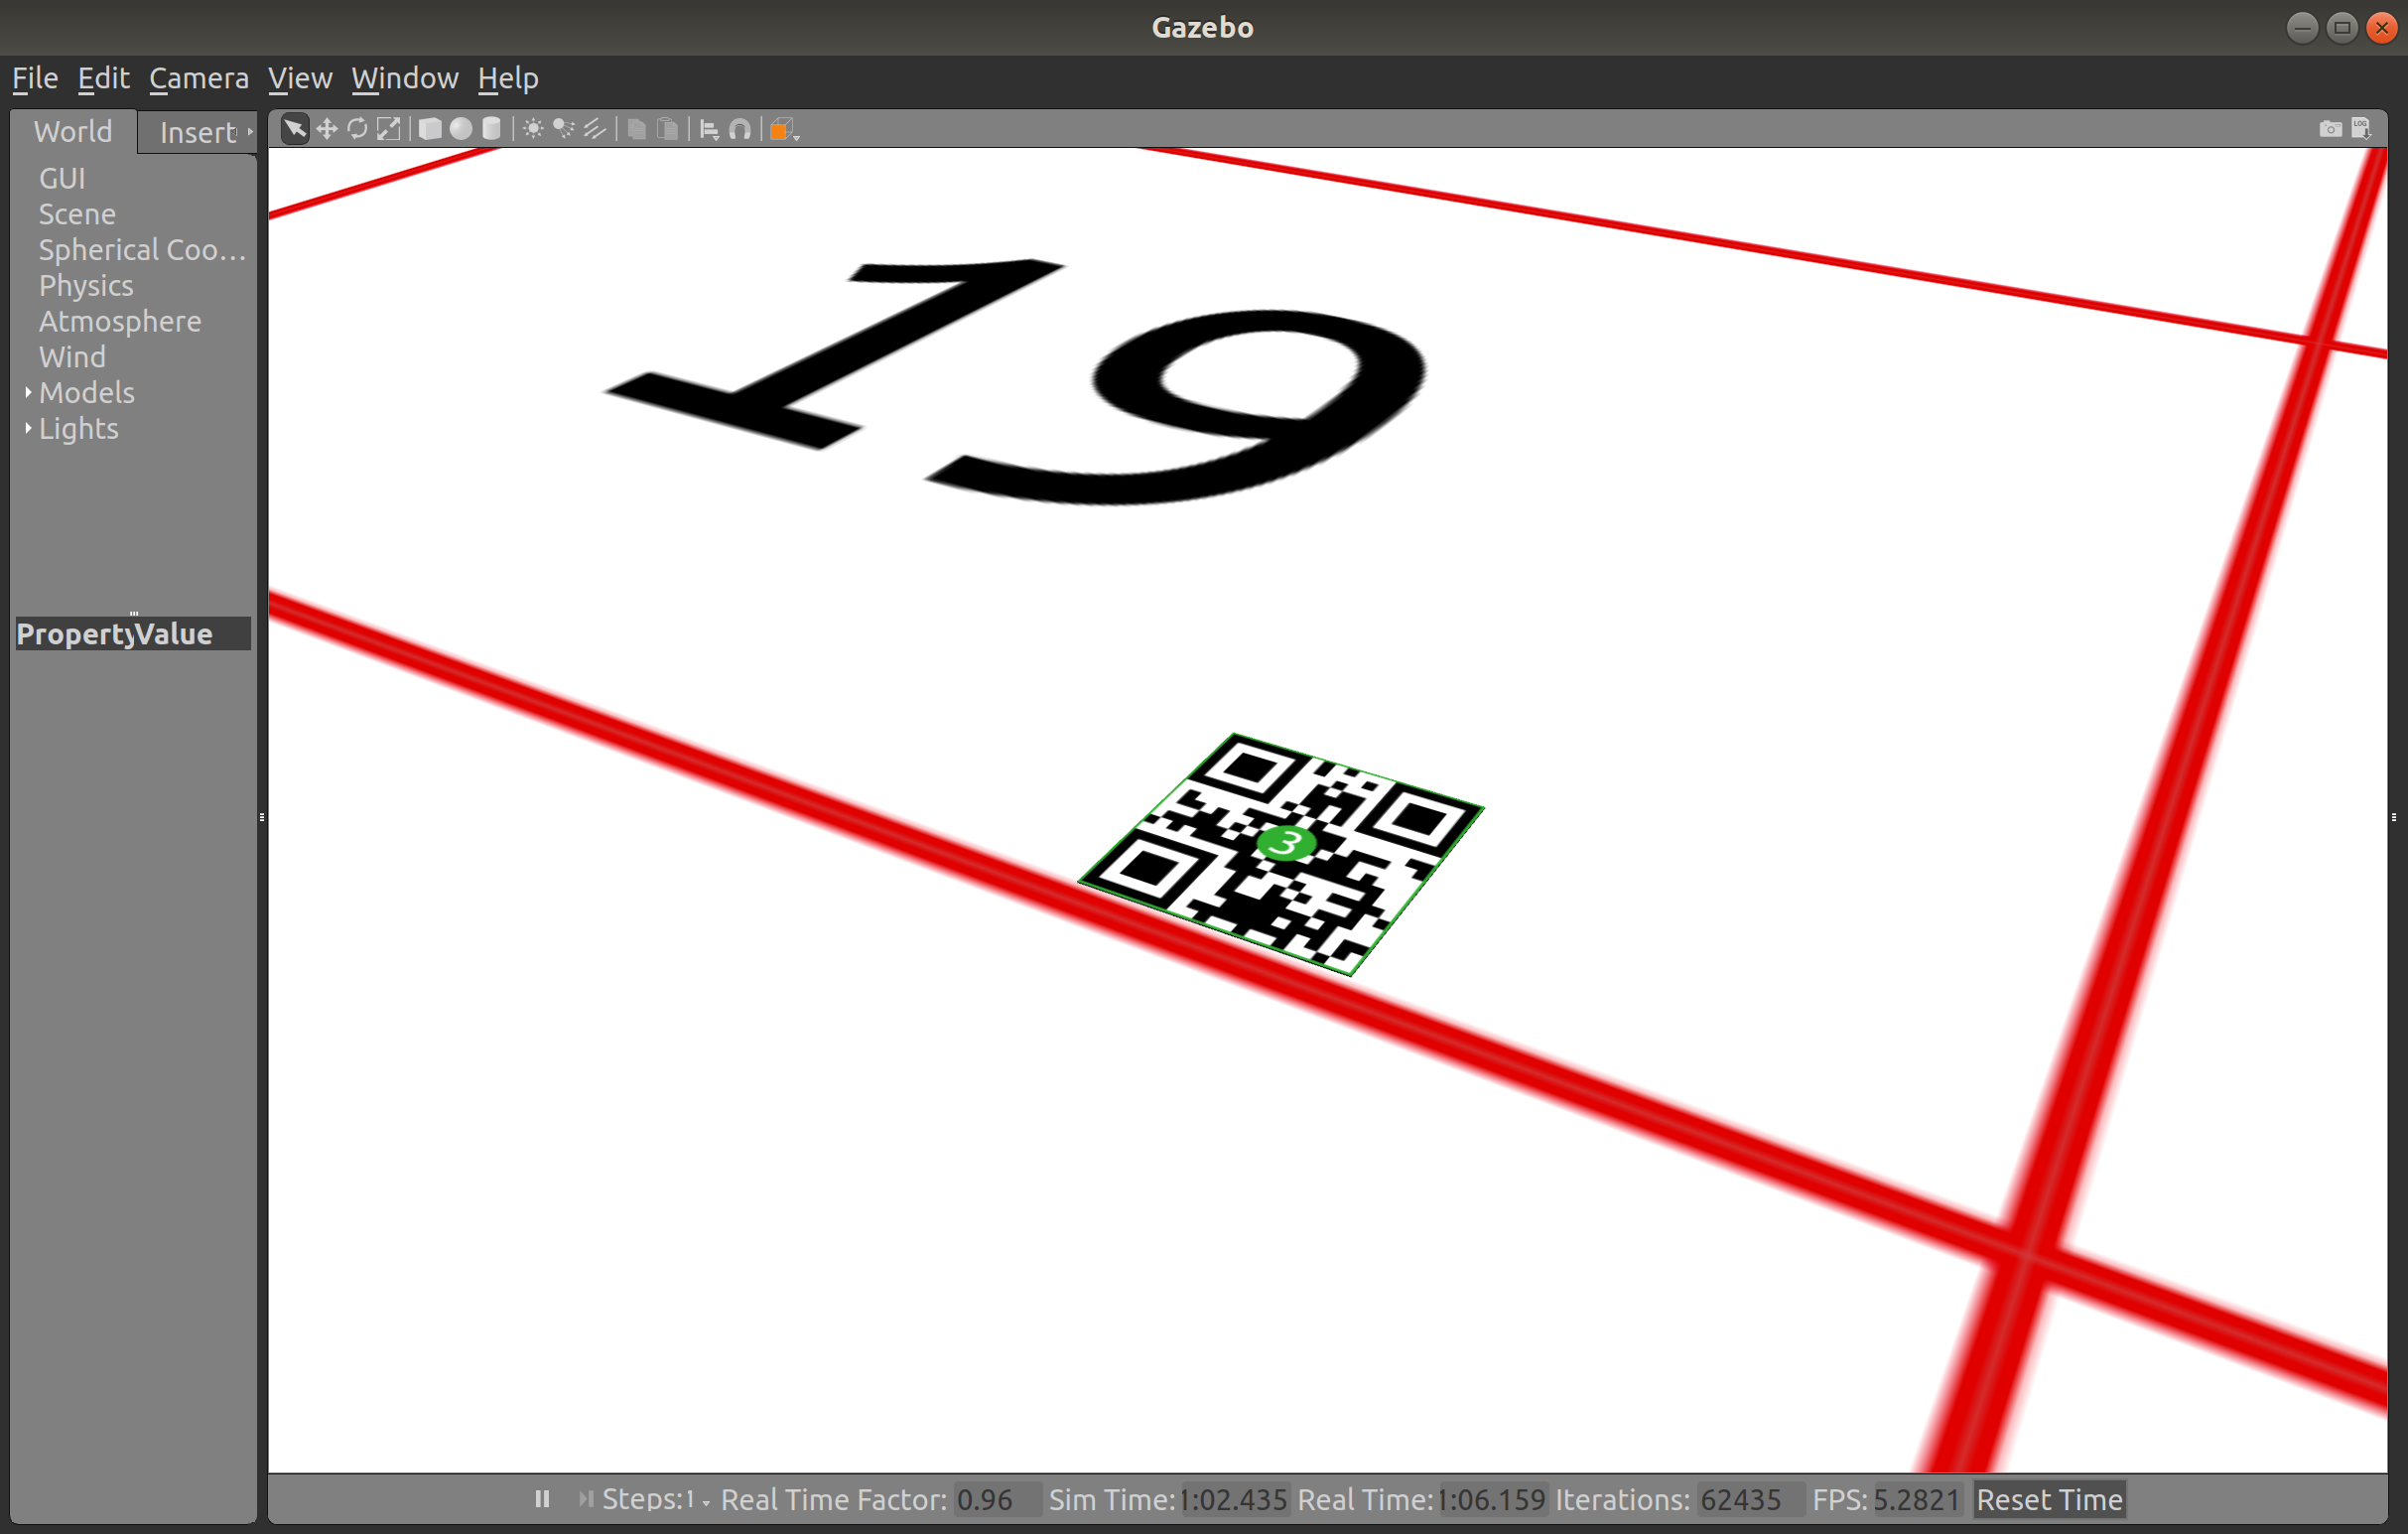
\includegraphics[width=0.8\textwidth]{target-3}
	\caption{Example of a target with ID 3 in the environment. The QR code
		embedding the ID information covers the top side of the target.}
	\label{fig:target}
\end{figure}

For the state space, the ground is divided into 25 cells as
illustrated in~\cref{fig:grid} with the numbers representing their
\textsc{id}s. 
In each timestep, the drone can occupy only one of these cells.
In addition to the cell \textsc{id}, the state space is made up of
other pieces of information as follows
\begin{align}
	s = \{ t, cell, [ I_1, I_2, I_3, \ldots, I_m] \} 
	\label{eq:state-space}
\end{align}

\noindent 
where $t$ is the current time step, $cell$ is the ID of the
cell underneath the drone, $I_k$ is the binary variable 
that indicates if the target with an ID of $k$ has been
visited, $m$ is the total number of targets,
and the vector of length $m$ is the container for the
$I$ indicators. 
For example,
if only targets with ID's 3 and 7 have been visited
in the current and previous time steps since the beginning of the 
episode,
then the vector will have elements of one for $I_3$ and $I_7$ while
the other elements are zeros.

\begin{figure}[!t]
	\centering
	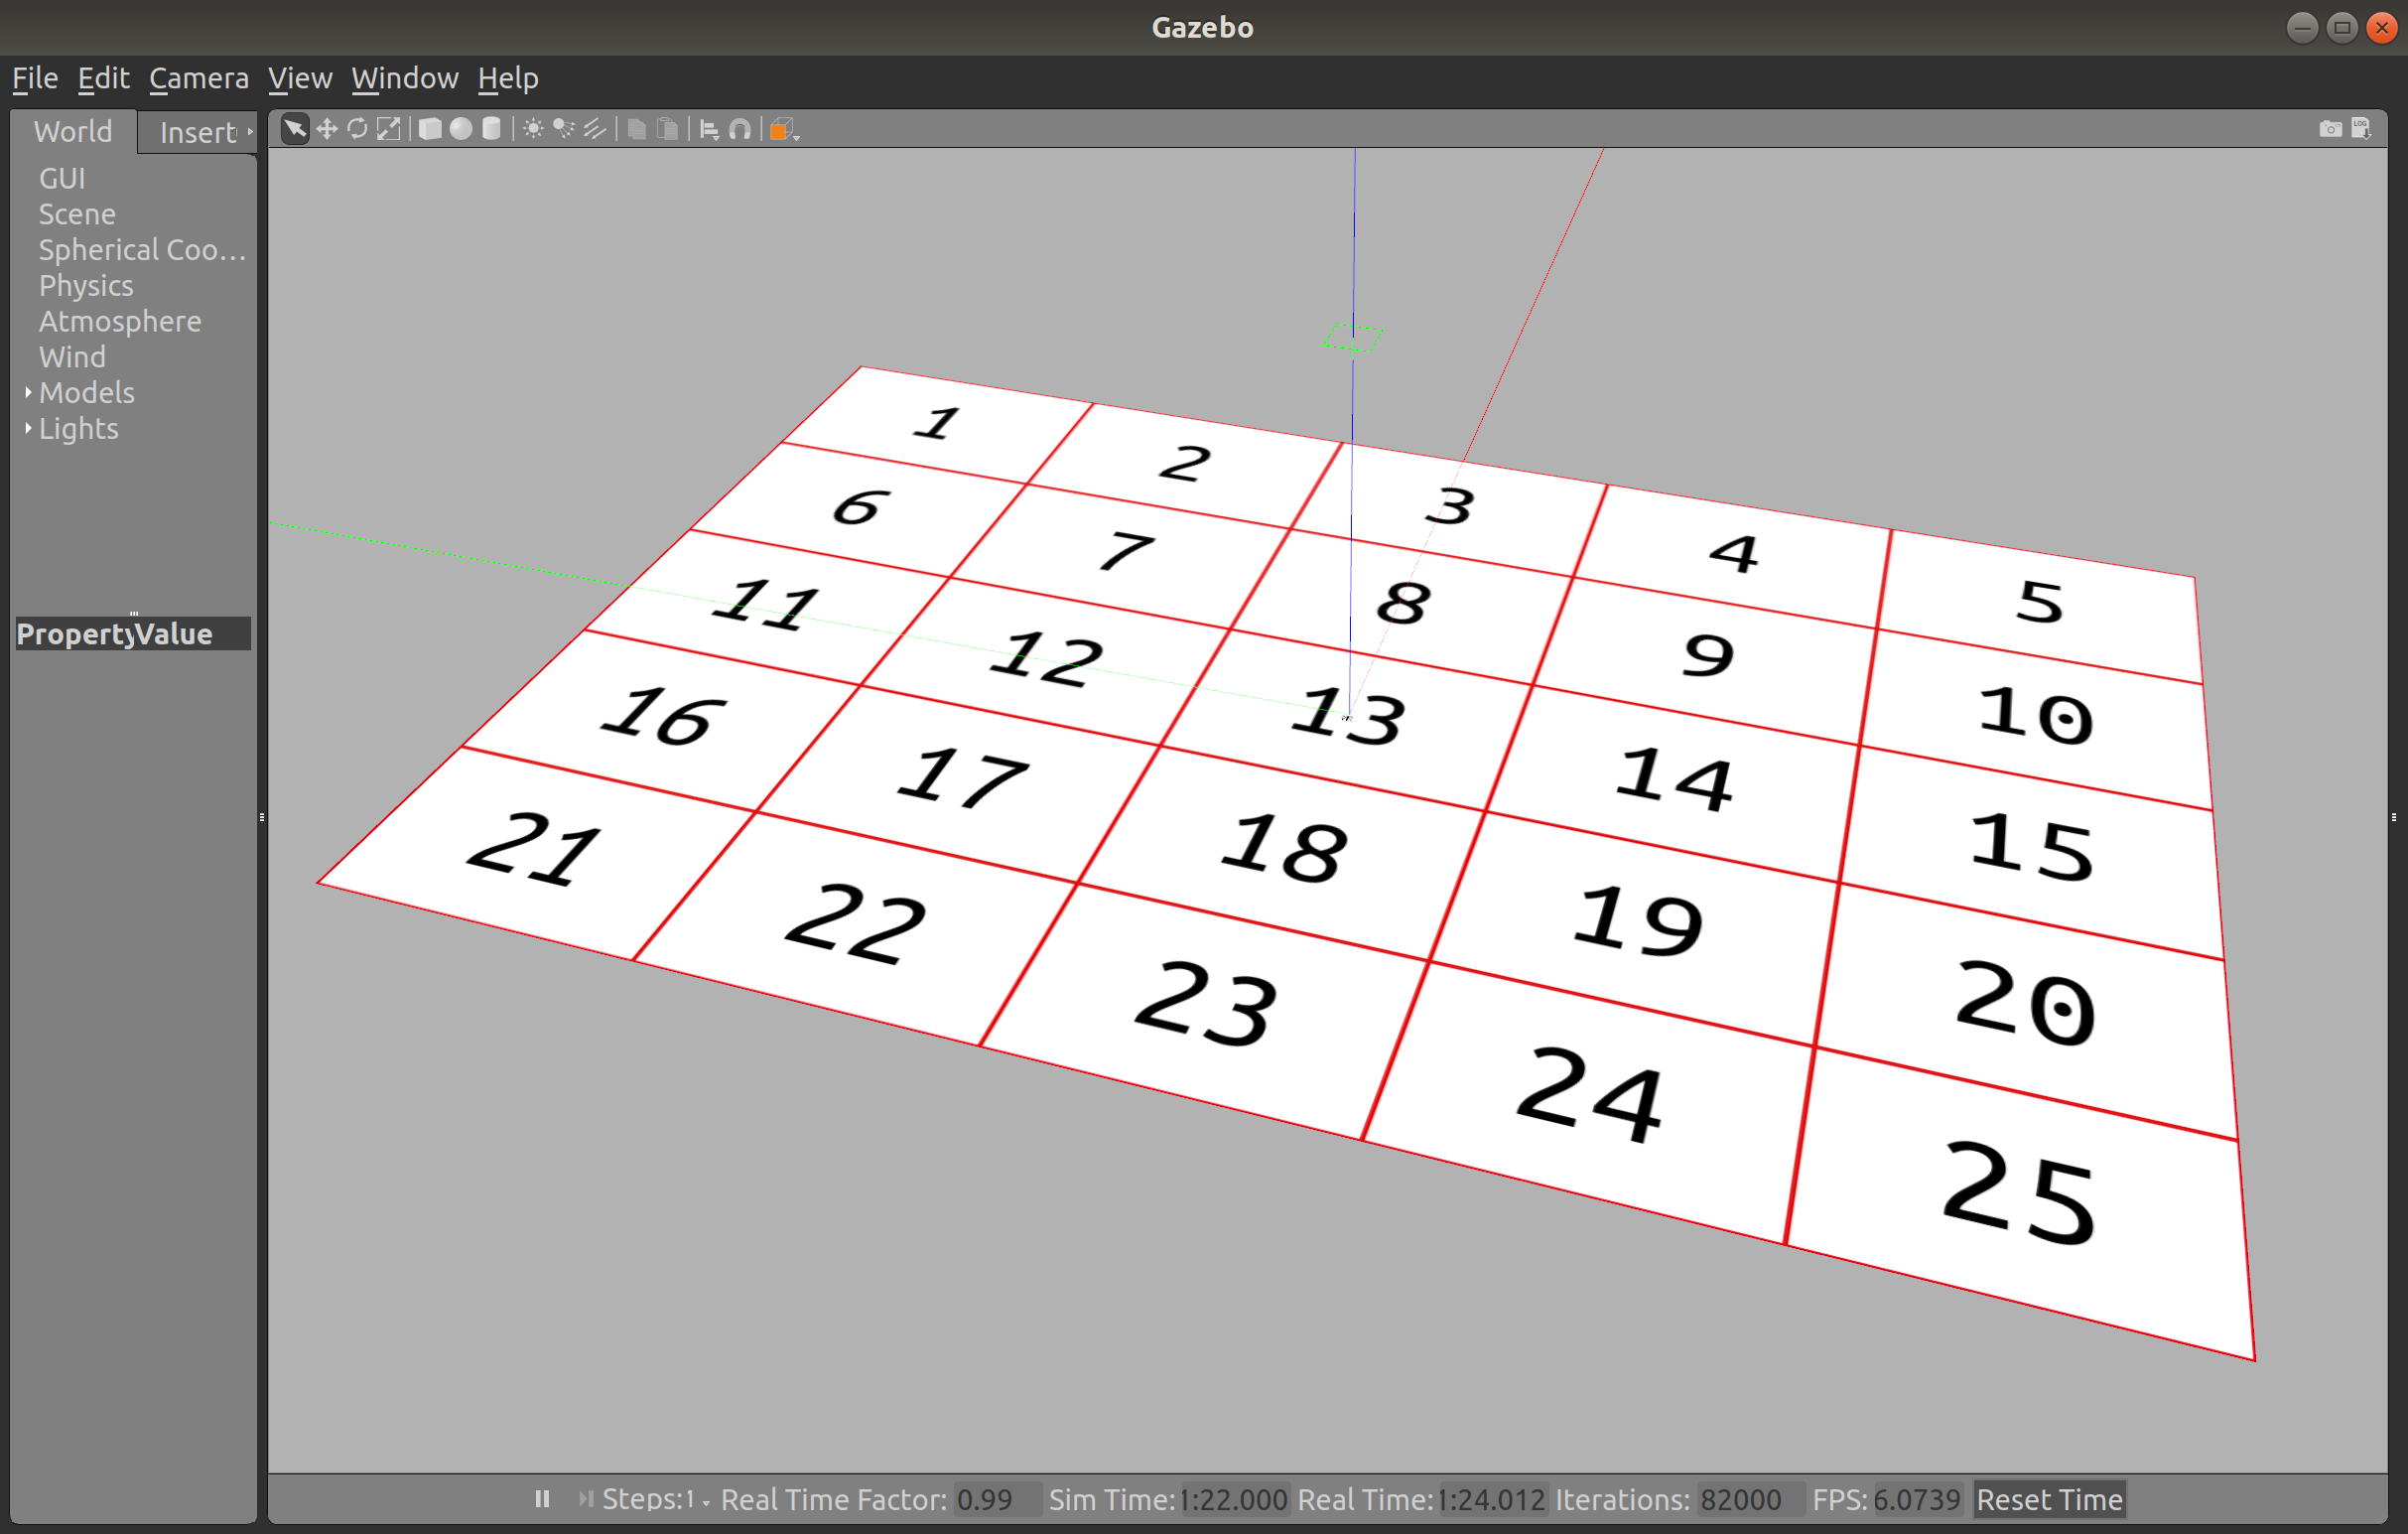
\includegraphics[width=0.8\textwidth]{grid}
	\caption{The environment of the agent with its ground
		divided into 25 cells.}
	\label{fig:grid}
\end{figure}

\subsubsection{User Interface}

We created a simple graphical user interface that allows an authorized user 
to connect to the drone, run different scripts on it, and even watch the live 
stream from the drone's camera. 
As illustrated in \cref{fig:gui-environments}, the solution is mainly a simple 
website that was built using html, css, and javascript for the frontend. As 
for the backend, we relied on Python Flask as the web framework due to 
its simplicity and practicality. Moreover, using Flask was beneficial for us 
because it is a lightweight framework with a built-in development server and a 
fast debugger provided. 
We relied on a web server gateway interface (\textsc{wsgi}) \textsc{http} 
server called Gunicorn which can forward requests to other web applications 
and frameworks that are written in Python.
Nginx is used as a reverse proxy server to ensure the smooth flow 
of traffic in the network. ZeroMQ was used to stream live videos from the 
Parrot Olympe framework to the flask web application using tcp/ip protocol. 
We used ZeroMQ because it is fast and lightweight. Also it is cross platform
and supports cross languages.

\begin{figure}[tbp] 
	\centering
	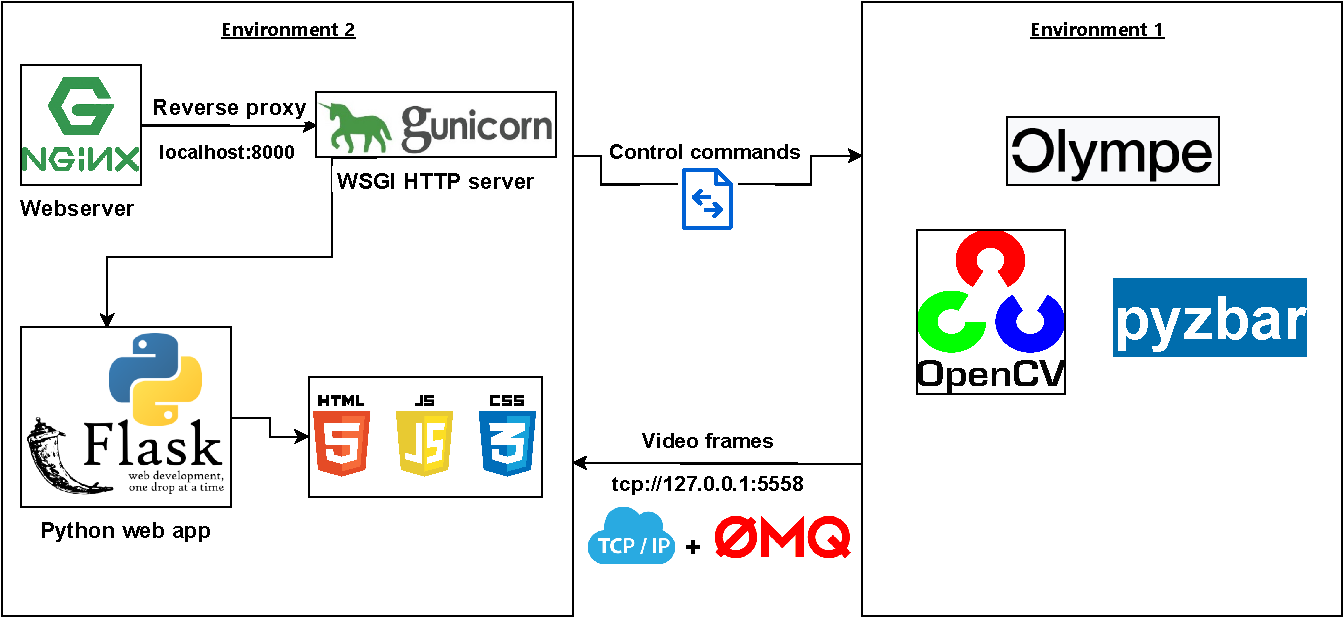
\includegraphics[width=0.9\textwidth]{gui-environments} 
	\caption{shows the interactions between software components that were included to 
		build the web-based \textsc{gui}.}
	\label{fig:gui-environments}  
\end{figure}


\end{document}
